\documentclass[
	12pt,				% tamanho da fonte
	openany,			% capítulos começam em pág ímpar (insere página vazia caso preciso)
	oneside, 			% oneside - twoside
	a4paper,			% tamanho do papel.
	chapter=TITLE,		% títulos de capítulos convertidos em letras maiúsculas
	section=TITLE,		% títulos de seções convertidos em letras maiúsculas
	sumario=tradicional,	
	%subsection=TITLE,	% títulos de subseções convertidos em letras maiúsculas
	%subsubsection=TITLE,% títulos de subsubseções convertidos em letras maiúsculas
	english,			% idioma adicional para hifenização
	brazil,				% o último idioma é o principal do documento
	]{abntex2}

% ---------------------------------------------------------------------------
% Inclui os comandos do projeto
% ---------------------------------------------------------------------------
\input{tex/commands}

% ---------------------------------------------------------------------------
% IDENTIFICAÇÃO
% ---------------------------------------------------------------------------
\titulo{Desenvolvimento dirigido por comportamento aplicado em um sistema simulado de travamento de portas veicular}
\autor{Robson Luan do Nascimento de Sousa}
\local{Santa Inês - MA}
\orientador{Prof. Emanuel Cleyton Macedo Lemos, Msc.}
\coorientador{Prof. Aristoteles de Almeida Lacerda Neto, Dr.}
%\coorientador{M. Sc. Osvaldo Campelo de Mello Vasconselos}
\instituicao{
Instituto Federal do Maranhão
	\par
CURSO DE GRADUAÇÃO EM ENGENHARIA DE COMPUTAÇÃO}
\tipotrabalho{Trabalho de Conclusão de Curso}
\preambulo{Trabalho apresentado ao Instituto Federal do Maranhão, Campus Santa Inês, como requisito da obtenção do título de Bacharel em Engenharia de Computação.}


% -----------------------------------------------------------------------------
% CONFIGURACAO DO SUMARIO - by @Gabrielr2508
% Precisa estar aqui, por isso não foi para o commands.tex, não descobrimos o motivo, %caso saiba, por favor, faça um pull request! :D
% -----------------------------------------------------------------------------
% Secao primaria (Chapter) Caixa alta, Negrito, tamanho 12
\makeatletter
\renewcommand*{\l@chapter}[2]{%
  \l@chapapp{\uppercase{#1}}{#2}{\cftchaptername}}
\makeatother
% Secao secundaria (Section) Caixa baixa, Negrito, tamanho 12
\renewcommand{\cftsectionfont}{\uppercase} %ponha \rmfamily se quiser serifadas...

% Secao terciaria (Subsection) Caixa baixa, negrito, tamanho 12
\renewcommand{\cftsubsectionfont}{\bfseries}

% Secao quaternaria (Subsubsection) Caixa baixa, tamanho 12
\renewcommand{\cftsubsubsectionfont}{\normalfont}

% Seção quinaria (subsubsubsection) Caixa baixa, sem negrito, tamanho 12
\renewcommand{\cftparagraphfont}{\normalfont\itshape}

% Para possibilitar o uso de codigo
%\usepackage{minted}

\usepackage{float}
\usepackage{listings}
\usepackage{xcolor} % Para customizar cores

\lstset{
  language=Python,        % ou C, C++, Java, etc.
  basicstyle=\ttfamily\footnotesize,
  numbers=left,
  numberstyle=\tiny,
  stepnumber=1,
  numbersep=5pt,
  backgroundcolor=\color{gray!10},
  frame=single,
  breaklines=true,
  captionpos=b,
  tabsize=2
}

%% Possibilita o uso da lista de quadros
\usepackage{tocloft} % criar listas personalizadas

% ----- Definição de QUADRO -----
%\newcounter{quadro}
%\newlistof{listofquadros}{loq}{Lista de Quadros}
%\renewcommand{\cftlistofquadrospresnum}{Quadro }
%\renewcommand{\cftlistofquadrosaftersnum}{ – }

% \newenvironment{quadro}[2][]{%
%     \refstepcounter{quadro}
%     \addcontentsline{loq}{quadro}{\protect\numberline{\thequadro}#2}
%     \begin{table}[H]
%     \centering
%     \caption*{Quadro \thequadro – #2} % legenda exibida
%     \ifx\\#1\\\else\label{#1}\fi
% }{%
%     \end{table}
% }



% -----------------------------------------------------------------------------
% Início do TCC 
% -----------------------------------------------------------------------------
\begin{document}

	\frenchspacing % Retira espaço extra obsoleto entre as frases.
	
	\pretextual
		%--------------------------------------------------------------------------------
% Constrói a capa com base na seção de identificação do main.tex
%--------------------------------------------------------------------------------
\begin{capa}
    \setlength{\belowcaptionskip}{0pt}
    \setlength{\abovecaptionskip}{0pt}
    \setlength{\intextsep}{-18pt}
        \begin{figure}[h]
    		\begin{center}
    		    
\includegraphics[scale=.5]{img/ifma_novo.jpg}
    		\end{center}
    	\end{figure}

        %\includegraphics[scale=0.6]{img/univasf.jpg}
        \center
    	{\ABNTEXchapterfont\large\imprimirinstituicao}

    	\vspace*{2cm}
    	    {\imprimirautor}
    	\vspace*{2cm}
        \begin{center}
    		\ABNTEXchapterfont\bfseries\large\imprimirtitulo
        \end{center}
    	\vfill

    	\ABNTEXchapterfont\bfseries\large\imprimirlocal\\
    	\the\year

    	\vspace*{1cm}
\end{capa}
%--------------------------------------------------------------------------------
% Constrói a folha de rosto com base na seção de identificação do main.tex
%--------------------------------------------------------------------------------
\begin{folhaderosto}
    \center
    	{\ABNTEXchapterfont\large\imprimirinstituicao}

		\vspace*{2cm}
    	    {\imprimirautor}
    	\vspace*{2cm}
		\vspace*{\fill}

		{\ABNTEXchapterfont\bfseries\large\imprimirtitulo}
		\vspace*{\fill}

		{\hspace{.45\textwidth}
		\begin{minipage}{.5\textwidth}
			\SingleSpacing
			\imprimirpreambulo \\ \\

			{\imprimirorientadorRotulo~\imprimirorientador\par}
			{\imprimircoorientadorRotulo~\imprimircoorientador\par}

		\end{minipage}%
		\vspace*{\fill}}%
		\vspace*{\fill}
			\ABNTEXchapterfont\bfseries\large\imprimirlocal\\
			\the\year
		\vspace*{1cm}
\end{folhaderosto}

%--------------------------------------------------------------------------------
% Constrói a ficha catalográfia com base na seção de identificação do main.tex
% Está comentado porque no final das contas a biblioteca do seu campus que gera a
% numeração, você pode adicionar os numeros aqui, ou anexar o pdf gerado por eles
% ao documento.
%--------------------------------------------------------------------------------
%\begin{fichacatalografica}
%	\vspace*{\fill}					% Posição vertical
%	\hrule							% Linha horizontal
%	\begin{center}					% Minipage Centralizado
%	\begin{minipage}[c]{12.5cm}		% Largura
%
%	\imprimirautor
%
%	\hspace{0.5cm} \imprimirtitulo  / \imprimirautor. --
%	\imprimirlocal, \the\year-
%
%	\hspace{0.5cm} xx p. : il. (algumas color.) ; 30 cm.\\
%
%	\hspace{0.5cm} \imprimirorientadorRotulo~\imprimirorientador\\
%
%	\hspace{0.5cm}
%	\parbox[t]{\textwidth}{\imprimirtipotrabalho~--~\imprimirinstituicao,
%	\the\year.}\\
%
%	\hspace{0.5cm}
%		1. Palavra-chave1.
%		2. Palavra-chave2.
%		I. Orientador.
%		II. Universidade xxx.
%		III. Faculdade de xxx.
%		IV. Título\\
%
%	\hspace{8.75cm} CDU 02:141:005.7\\
%
%	\end{minipage}
%	\end{center}
%	\hrule
%\end{fichacatalografica}

%--------------------------------------------------------------------------------
% Anexando a ficha catalogáfica e a folha de aprovação
%--------------------------------------------------------------------------------
\includepdf[pages=-]{anexos/ficha.pdf}

\includepdf[pages=-]{anexos/aprovacao.pdf}

\setlength{\ABNTEXsignwidth}{12cm}

%--------------------------------------------------------------------------------
% Está comentado pelo mesmo motivo da ficha catalográfica
%--------------------------------------------------------------------------------
%\begin{folhadeaprovacao}
%	\begin{center}
%	    {\ABNTEXchapterfont\bfseries\large\imprimirinstituicao}
%	    \vspace*{\fill}
%
%	    {\ABNTEXchapterfont\bfseries\large FOLHA DE APROVAÇÃO}
%	    \vspace*{\fill}
%
%	    {\ABNTEXchapterfont\bfseries\large\imprimirautor}
%
%	    \vspace*{\fill}\vspace*{\fill}
%	    {\ABNTEXchapterfont\bfseries\large\imprimirtitulo}
%	    \vspace*{\fill}
%
%	    {\hspace{.45\textwidth}
%		\begin{minipage}{.5\textwidth}
%			\SingleSpacing
%			\ABNTEXchapterfont\imprimirpreambulo \\ \\
%
%			{\ABNTEXchapterfont\imprimirorientadorRotulo~\imprimirorientador\par}
%			{\ABNTEXchapterfont\imprimircoorientadorRotulo~\imprimircoorientador\par}
%
%		\end{minipage}%
%	    \vspace*{\fill}}
%	\end{center}
%
%	\vspace*{\fill}
%
%	\begin{center}
%			 \ABNTEXchapterfont\large Aprovado em: \_\_\_\_ de \_\_\_\_ de 2017
%	\end{center}

%	\vspace*{\fill}

%	\begin{center}
%			 \ABNTEXchapterfont\bfseries\large Banca Examinadora
%	\end{center}
%
%   \ABNTEXchapterfont\assinatura{Fábio Nelson de Sousa Pereira, Mestre, Universidade Federal do Vale do São Francisco}
%	\ABNTEXchapterfont\assinatura{Jorge Luis Cavalcanti Ramos, Doutor, Universidade Federal do vale do São Francisco}
%  \ABNTEXchapterfont\assinatura{Ricardo Argenton Ramos, Doutor, Universidade Federal do Vale do São Francisco}
%	 \vspace*{\fill}


%\end{folhadeaprovacao}

%--------------------------------------------------------------------------------
% Insere a epígrafe
%--------------------------------------------------------------------------------
\newpage
\vspace*{\fill}
\begin{flushright}
		\textit{Lorem Ipsum...}
\end{flushright}

%--------------------------------------------------------------------------------
% Seção de agradecimentos
%--------------------------------------------------------------------------------
\begin{agradecimentos}

\lipsum[2-4]

\end{agradecimentos}

%--------------------------------------------------------------------------------
% Insere a segunda epígrafe
%--------------------------------------------------------------------------------
\begin{epigrafe}
    \vspace*{\fill}
	\begin{flushright}
		Se pude enxergar a tão grande distância, foi subindo nos ombros de gigantes.\\
		 \vspace{\baselineskip}
		\textbf{Isaac Newton}\\
		\textbf{Carta à Robert Hooke, 1676}
	\end{flushright}
\end{epigrafe}



%--------------------------------------------------------------------------------
% Seção de resumos
%--------------------------------------------------------------------------------
% resumo em português
\setlength{\absparsep}{18pt} % ajusta o espaçamento dos parágrafos do resumo
\begin{resumo}

\lipsum[1-2]

 \textbf{Palavras-chave}: \textit{Palavra em inglês 1, Palavra em inglês 2, Palavra em inglês 3, Palavra em inglês 4}, Palavra 5.

\end{resumo}

%---------------------------------------------------------------------------------
% resumo em inglês
\begin{resumo}[Abstract]
\begin{otherlanguage*}{english}

\lipsum[3-4]

	\vspace{\onelineskip}

	\noindent
	\textbf{Key-words}: \textit{Palavra em inglês 1, Palavra em inglês 2, Palavra em inglês 3, Palavra em inglês 4, Palavra em inglês 4}.

\end{otherlanguage*}
\end{resumo}


%---------------------------------------------------------------------------------
% Insere lista de ilustrações
%---------------------------------------------------------------------------------
\begin{KeepFromToc} % Este comando evita que todas as seções dentro dele de apareçam no sumário
\pdfbookmark[0]{\listfigurename}{lof}
\listoffigures
%\addcontentsline{toc}{chapter}{Lista de Figuras}
\cleardoublepage


%---------------------------------------------------------------------------------
% Insere lista de tabelas
%---------------------------------------------------------------------------------
\pdfbookmark[0]{\listtablename}{lot}
\listoftables
\cleardoublepage

%---------------------------------------------------------------------------------
% Insere lista de quadros
%---------------------------------------------------------------------------------
\pdfbookmark[0]{\listofquadrosname}{loq}
\listofquadros*
\cleardoublepage

%---------------------------------------------------------------------------------
% Ajusta lista de código - alterar de figures para códigos - by @Gabrielr2508
%---------------------------------------------------------------------------------
\makeatletter
\let\l@listing\l@figure
\def\newfloat@listoflisting@hook{\let\figurename\listingname}
\makeatother

%---------------------------------------------------------------------------------
% Insere lista de códigos - by @leolleocomp
%---------------------------------------------------------------------------------
\listoflistings

\end{KeepFromToc}

%---------------------------------------------------------------------------------
% Insere lista de abreviaturas e siglas
%---------------------------------------------------------------------------------
\begin{siglas}
	\item[LI]       Lorem Ipsum
    \item[LII]		Lorem Ipsum Ipsum

\end{siglas}

%---------------------------------------------------------------------------------
% Insere o sumario
%---------------------------------------------------------------------------------
\pdfbookmark[0]{\contentsname}{toc}
\tableofcontents*
\cleardoublepage




	\textual
		\pagestyle{simple}
		%--------------------------------------------------------------------------------------
% Este arquivo contém a sua introdução, objetivos e organização do trabalho
%--------------------------------------------------------------------------------------
\chapter{Introdução}

A indústria automotiva tem experimentado um crescimento constante, acompanhado por um aumento significativo na modernização dos veículos e pela intensa competição entre 
montadoras para entregar produtos cada vez mais robustos e de alta qualidade. Esse cenário traz consigo um aumento na complexidade do desenvolvimento, demandando soluções 
mais eficientes e seguras para sistemas cada vez mais sofisticados e que sejam capazes de atender às necessidades específicas de cada cliente.

A modernização do setor automotivo tem conduzido ao próximo grande avanço: os veículos definidos por software (\textit{Software-Defined Vehicles}) 
\cite{softwareVehicles2025}. Essa abordagem possibilita a customização contínua e a evolução do produto mesmo após a aquisição, permitindo a entrega de novas 
funcionalidades ao veículo por meio de atualizações de software feitas remotamente \textit{Over-the-Air (OTA)}, suportadas pelo hardware já embarcado.

Diante desse contexto, a Engenharia Automotiva enfrenta o desafio de projetar e desenvolver produtos com um nível altíssimo de qualidade, ao mesmo tempo em que busca reduzir 
erros e retrabalho. A aplicação de metodologias ágeis, como o \textit{Behavior Driven Development (BDD)} \cite{north2006bdd}, oferece uma abordagem promissora, pois foca na 
definição do comportamento esperado do sistema a partir da perspectiva do usuário. Essa abordagem permite uma colaboração mais efetiva entre os membros de uma equipe ágil 
\cite{atlassianAgileTeams}, facilita a descoberta de funcionalidades e possibilita que o desenvolvimento seja guiado por testes de aceitação automatizados, promovendo 
entregas de valor de forma mais rápida e com maior confiabilidade.

\section{\textbf{Justificativa}}

O problema central deste trabalho é: ``como é possível aplicar o processo de BDD para facilitar a definição do sistema e guiar seu desenvolvimento no contexto da 
Engenharia de Sistemas Automotivos?''. A solução proposta consiste na adaptação do processo, integrando as técnicas já consolidadas do BDD com metodologias 
amplamente utilizadas na indústria automotiva, de forma a lidar com as complexidades inerentes ao desenvolvimento de sistemas veiculares.

Este trabalho insere-se no contexto atual da indústria automotiva, adotando o sistema de travamento de portas como prova de conceito para a geração do produto. 
Durante seu desenvolvimento, serão consideradas como referência implementações reais de sistemas já presentes em veículos, como os da Volkswagen \cite{vwLocking} 
e da Bosch \cite{bosch2022handbook,reif2017locking}. Nesse sentido, a adaptação do processo de BDD será aplicada ao desenvolvimento de um produto compatível com 
as especificações industriais, ao mesmo tempo em que busca minimizar as complexidades enfrentadas em sua execução.

O BDD incorpora diversas premissas que surgem das lições aprendidas na aplicação de outras metodologias ágeis, definindo o desenvolvimento do produto a partir do 
comportamento que gera valor ao usuário. Além disso, ele busca promover a colaboração entre as diferentes etapas do desenvolvimento, garantindo que toda a equipe 
compreenda o produto e consiga assumir a perspectiva do usuário.

Por outro lado, a Engenharia Automotiva apresenta uma complexidade significativa, o que torna desafiadora a entrega de produtos de alta qualidade. A definição de 
um sistema veicular envolve muito mais do que software ou eletrônica, sendo necessário integrar componentes mecânicos, considerar falhas 
potenciais, garantir a rastreabilidade de requisitos e contemplar casos de uso extremos.

O principal desafio deste trabalho consiste em identificar técnicas capazes de capturar as complexidades envolvidas no desenvolvimento de sistemas automotivos 
e adaptá-las às premissas do BDD. Em casos como o do sistema de travamento de portas, isso é traduzido na necessidade de atender a funcionalidades 
essenciais, como (GSMH, 2022):

\begin{itemize}
    \item Permitir o acesso ao interior do veículo para todas as pessoas autorizadas;
    \item Gerenciar a abertura das portas a partir das maçanetas internas e externas;
    \item Proteger os ocupantes da abertura indevida das portas;
    \item Proteger o veículo contra furtos enquanto ele está estacionado.
\end{itemize}

Uma das principais complexidades desse tipo de sistema está na definição do mecanismo empregado no travamento das portas. Conforme descrito por 
\citeonline{reif2017locking}, podem ser utilizadas travas mecânicas ou eletrônicas, cada um com conjuntos específicos de componentes e lógicas de 
software distintas que influenciam diretamente o desenvolvimento. Esse desafio é recorrente na indústria automotiva, na qual diversos sistemas dependem 
de decisões técnicas de hardware ou soluções mecânicas para viabilizar o início do processo de design.

Neste trabalho, será apresentada uma metodologia que demonstra como a aplicação do Desenvolvimento Orientado a Comportamento (BDD) possibilita projetar o 
sistema de forma independente dos detalhes técnicos, facilitando tanto o desenvolvimento das funcionalidades quanto a execução dos testes. Isso ocorre 
porque a abordagem do BDD prioriza a perspectiva do usuário e a especificação do comportamento esperado do sistema, os quais não estão diretamente vinculados 
à implementação.

\section{\textbf{Objetivos}}

\subsection{Objetivo Geral}
%Para responder à problemática levantada, o presente estudo tem como objetivo geral 
Aplicar o levantamento e definição de funcionalidades na análise de um sistema de travamento de portas veicular, seguido do desenvolvimento guiado por testes de 
aceitação automatizados, demonstrando como essas práticas podem contribuir para o desenvolvimento de software automotivo de forma mais organizada e eficiente.

\subsection{Objetivos Específicos}
\begin{itemize}
    \item Realizar o levantamento e definição de funcionalidades considerando possíveis limitações decorrentes da dependência de hardware e de sistemas mecânicos;
	\item Analisar as complexidades dos sistemas automotivos de maneira compatível com o processo de BDD;
    \item Empregar técnicas de desenvolvimento como padrão de escrita de software AUTOSAR \cite{autosarClassic} e Design Orientado por Modelos (\textit{Model-Based Desgin - MBD}) \cite{mathworksMBD2024}, que são amplamente utilizadas na indústria automotiva;
    \item Definir um escopo de desenvolvimento que possibilite a realização do design do sistema forma clara e compreensível;
    \item Empregar testes de aceitação automatizados para guiar o desenvolvimento do sistema, consistente com o design definido;
    \item Realizar a implementação do sistema de maneira iterativa, possiblitando à descoberta de melhorias surgidas durante a aplicação do processo;
    \item Aplicar a metodologia desenvolvida na produção de um sistema de travamento de portas veicular simulado.
\end{itemize}

% \section{Metodologia}

% A metodologia utilizada neste estudo baseia-se na revisão da bibliografia disponível, com o objetivo de esclarecer o processo de BDD e investigar como ele pode 
% ser adaptado para incorporar práticas consolidadas na Engenharia Automotiva. Para tanto, serão aplicadas técnicas como o mapeamento de exemplos 
% \cite{Lawrence2019cucumber, cucumberExampleMapping}
% , voltado ao levantamento e definição de funcionalidades, e testes de aceitação automatizados 
% \cite{studyBDD}
% , que servirão para guiar o desenvolvimento do sistema.

% A implementação do sistema simulado também fará uso de técnicas típicas da Engenharia Automotiva, incluindo o Model Based Design
% \cite{Vincentelli2001, mathworksMBD2024} e a geração automática de código segundo o padrão de software AUTOSAR 
% \cite{autosarClassic}. Conceitos adicionais do domínio automotivo serão considerados para 
% assegurar a adequada abstração nas diferentes etapas do desenvolvimento.

% Espera-se que os resultados obtidos evidenciam os benefícios da integração do BDD no contexto automotivo, destacando sua contribuição para a qualidade e 
% confiabilidade do sistema. A validação será realizada por meio da execução dos testes de aceitação e da análise do uso do sistema final sob a perspectiva do usuário.

\section{\textbf{Organização do trabalho}}
No Capítulo \ref{ch:te}, serão apresentados os conceitos que compõem a fundamentação teórica deste trabalho, abrangendo:

\begin{itemize}
    \item \textbf{O processo de BDD} - histórico do desenvolvimento do processo e seus pilares fundamentais do processo;
    \item \textbf{Mapeamento de exemplos} - metodologia aplicada para realizar a análise do sistema e definição de funcionalidades;
    \item \textbf{A linguagem \textit{Gherkin}} - linguagem usada para a escrita de cenários, que atuam como definição de comportamentos e como testes de aceitação;
    \item \textbf{Design orientado por modelo} - metodologia adotada para a implementação do sistema;
    \item \textbf{Sistemas de travamento de porta veiculares} - definição e caracterização dos sistemas de segurança voltados ao travamento de portas em veículos. 
\end{itemize}

Em seguida, no Capítulo \ref{ch:MM}, será apresentada a metodologia adotada, descrevendo o procedimento de desenvolvimento do produto, estruturado em seis etapas. 
Serão também detalhadas as ferramentas utilizadas neste trabalho, bem como os critérios de avaliação, definidos a partir da execução dos testes de aceitação de 
cada funcionalidade do sistema.

No Capítulo \ref{ch:IM}, a implementação é conduzida por meio da execução das quatro primeiras etapas do processo. Essa fase tem início com a definição das histórias 
de usuário — que representam as funcionalidades do sistema — conforme descrito na Seção \ref{sbs:etapa1}. A histórias orientam todas as etapas subsequentes, desde a 
elaboração dos testes de aceitação até a modelagem do sistema.

Para cada história de usuário, o mapeamento de exemplos, descrito na Seção \ref{sbs:etapa2}, será empregado para orientar a definição dos detalhes relacionados 
ao comportamento esperado. Em seguida, na Seção \ref{sbs:etapa3}, o sistema será modelado como uma abstração que explicita as interações com o usuário, ao mesmo 
tempo em que oculta os aspectos técnicos de sua implementação. A partir das histórias de usuário e do modelo do sistema, será elaborada, na Seção \ref{sbs:etapa4}, 
uma série de cenários que representam tanto a especificação do comportamento esperado quanto os testes de aceitação correspondentes.  

No capítulo \ref{ch:RD}, será feita a execução dos testes de validação que foram criados ao fim do capítulo \ref{ch:IM}. Esse processo é feito para garantir 
que a modelagem do sistema é guiada a partir dos cenários desenvolvidos e satisfaz o comportamento definido como uma forma de resolver erros capturados na execução 
dos testes. 

No Capítulo \ref{ch:RD}, serão executados os testes de validação definidos pelos cenários das histórias de usuário. Esse processo assegura que a modelagem do sistema 
seja orientada pela execução dos testes e que o comportamento especificado seja atendido. Ela também possibilita a identificação e a correção de falhas detectadas 
durante a execução dos testes.

A aprovação das histórias de usuário será realizada a partir da verificação de que:

\begin{itemize}
    \item Os testes foram executados e confirmaram a aprovação de todos os cenários relacionados à história;
    \item A execução dos cenários é repetida ao longo do desenvolvimento das demais histórias, de modo a assegurar que o comportamento previamente validado não seja comprometido.
\end{itemize}

Por fim, no Capítulo \ref{ch:CC}, será apresentada uma síntese dos principais aspectos observados durante a aplicação da metodologia proposta. Adicionalmente, serão 
discutidas algumas limitações do escopo deste trabalho, acompanhadas de sugestões de continuidade para o desenvolvimento futuro que culminam na geração do produto físico.

		%--------------------------------------------------------------------------------------
% Este arquivo contém a sua funtamentação teórica
%--------------------------------------------------------------------------------------
\chapter{Fundamentação teórica}

\section{Seção de exemplo 1 - Como fazer citações}

Existem vários tipos de citações...


\section{Seção de exemplo 2 - Como inserir figuras}

Neste trabalho iremos exemplificar duas formas de se inserir figuras no Latex. O primeiro método insere, no documento, uma figura simples por meio do comando:

\textbackslash imagem\{ Escala \}\{ Arquivo sem extensão \}\{ Descrição \}\{ Fonte \}

\textbf{Obs.:} A fonte pode ser uma citação do tipo  \textbackslash citeonline\{\}.

% A figura \ref{img:placeholder} é um exemplo deste método.

% %--------------------------------------------------------------------------------------
% % Esse é um exemplo de figura simples
% %--------------------------------------------------------------------------------------
% \imagem{0.15}{placeholder}{Uma figura simples}{O autor}

% A figura \ref{img:figura1} é um exemplo do outro tipo de figura abordada aqui, chamada de figura composta. Esta figura é composta de outras subfiguras.
% %--------------------------------------------------------------------------------------
% % Esse é um exemplo de figura composta de outras subfiguras
% %--------------------------------------------------------------------------------------
% \begin{figure}[!htb]
% \centering
%     \caption{\label{img:figura1} Exemplo de figura composta}
%     \subcaptionbox{\label{img:subfigura1} Subfigura 1}{\includegraphics[scale=.1]{img/placeholder}}\qquad
%     \subcaptionbox{\label{img:subfigura2} Subfigura 2}{\includegraphics[scale=.1]{img/placeholder}}
%     \vspace{1.5em}
%     \legend{\textbf{Fonte:} \citeonline{SUA-REFERENCIA}}
% \label{fig:dag}
% \end{figure}

%\begin{figure}[!htb]
%\centering
%    \caption{\label{img:telas} Telas da aplicação cliente}
%    \subcaptionbox{\label{img:inicial} Abertura}{\includegraphics[scale=.12]{img/APP/inicial}}\qquad
%    \subcaptionbox{\label{img:login} \textit{Login}}{\includegraphics[scale=.12]{img/APP/login}}\qquad
%    \subcaptionbox{\label{img:cadastro} Cadastro}{\includegraphics[scale=.12]{img/APP/cadastro}}\qquad
%    \subcaptionbox{\label{img:hist-rel}Sobre}{\includegraphics[scale=.12]{img/APP/sobre}}\\
%    \vspace{1.5em}
%    \subcaptionbox{\label{img:dados_atuais}Dados atuais}{\includegraphics[scale=.15]{img/APP/atual}}\qquad
%    \subcaptionbox{\label{img:hist-time}Seleção de período}{\includegraphics[scale=.15]{img/APP/periodo}}\qquad
%    \subcaptionbox{\label{img:hist-rel}Exibir histórico}{\includegraphics[scale=.15]{img/APP/historico}}\\
%    \vspace{2.5em}
%    \legend{\textbf{Fonte:} O Autor}
%\label{fig:dag}
%\end{figure}

\begin{figure}[ht]
\centering
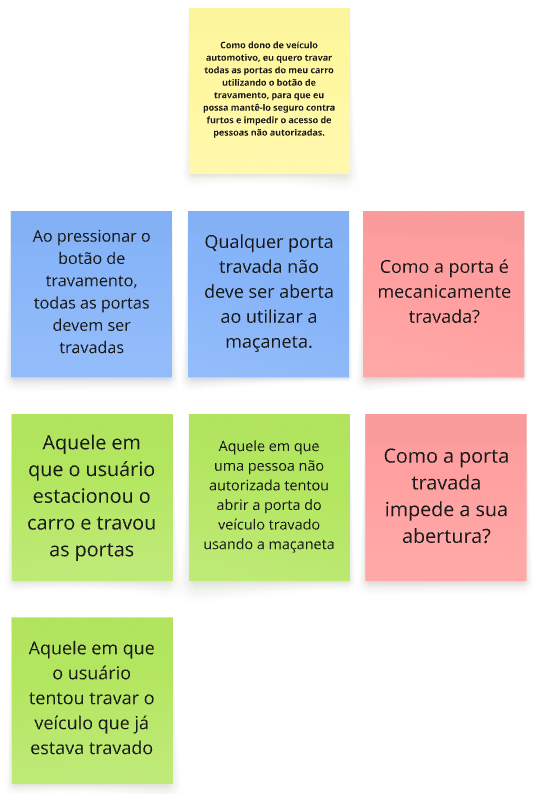
\includegraphics[height=12cm]{figuras/user_story_1.png}
\caption{História de Usuário 1: Travamento de todas as portas}
%\label{fig:casos-uso}
\end{figure}

\begin{figure}[ht]
\centering
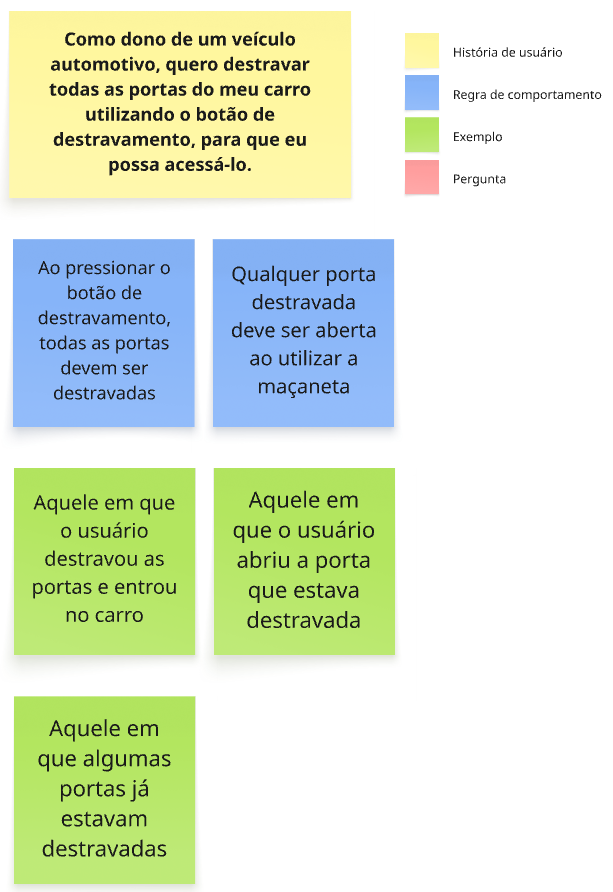
\includegraphics[height=12cm]{figuras/user_story_2.png}
\caption{História de Usuário 2: Destravamento de todas as portas}
%\label{fig:casos-uso}
\end{figure}

\begin{figure}[ht]
\centering
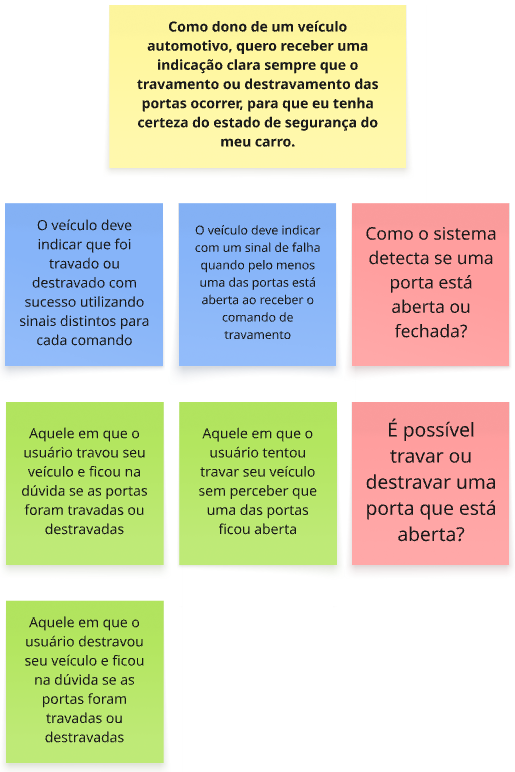
\includegraphics[height=12cm]{figuras/user_story_3.png}
\caption{História de Usuário 3: Feedback de travamento}
%\label{fig:casos-uso}
\end{figure}

\begin{figure}[ht]
\centering
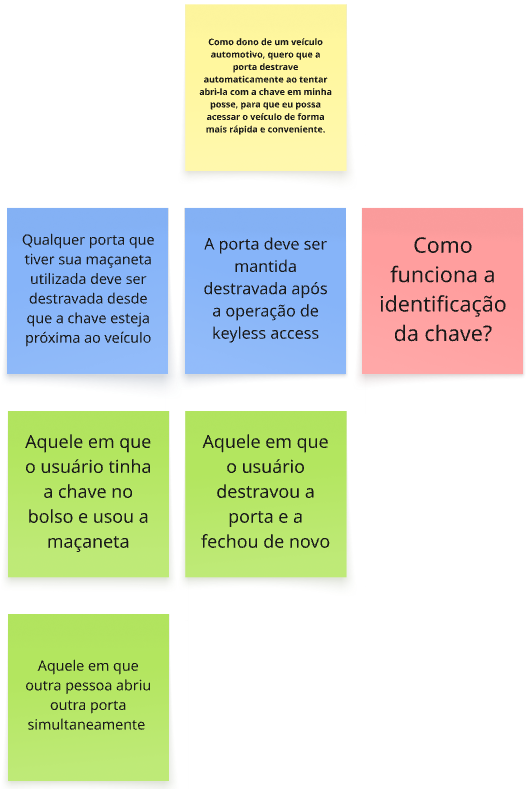
\includegraphics[height=12cm]{figuras/user_story_4.png}
\caption{História de Usuário 4: Keyless Access}
%\label{fig:casos-uso}
\end{figure}

\begin{figure}[ht]
\centering
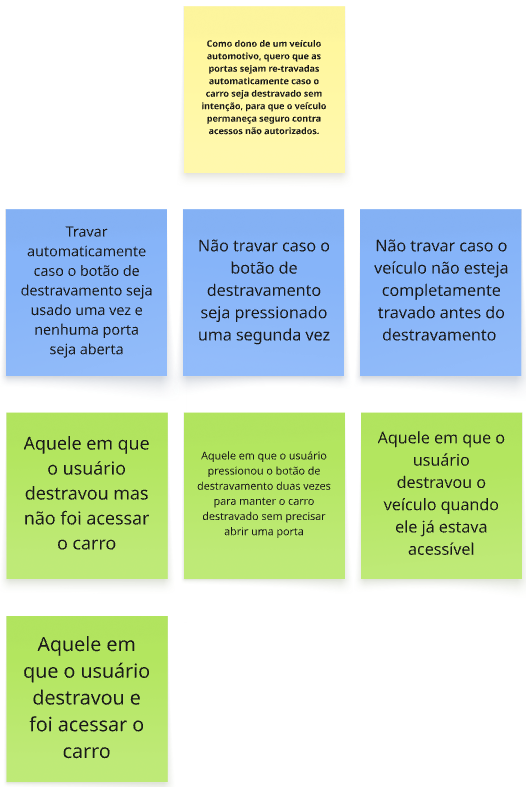
\includegraphics[height=12cm]{figuras/user_story_5.png}
\caption{História de Usuário 5: Travamento automático}
%\label{fig:casos-uso}
\end{figure}

Para referenciar uma figura deve ser usada comando \textbackslash ref\{img:<label ou nome do arquivo>\}, como exemplo, estamos referenciando a figura \ref{img:placeholder}. Isso vale tanto para figuras simples quanto para as compostas, como por exemplo as figuras \ref{img:subfigura1} e \ref{img:subfigura2}. Ao inserir uma figura, ela é automaticamente identificada e incluída no elemento pré-textual da lista de figuras.




\section{Seção de exemplo 3 - Sobre tabelas}

As tabelas em Latex são deveras capciosas, por isso não serão abordadas em sua completude neste documento.

Há um site que possui uma ferramenta interessante para ser utilizada na construção tabelas em Latex.

\centerline{\href{https://www.tablesgenerator.com/}{ O Tables Generator } <-- Isto é um \textit{link} :D}

Contudo, busquem entendimento sobre o assunto, pois tabelas são elementos textuais importantes e enriquecem muito o texto, quando bem construídas.

A tabela \ref{tab:crossplatform} é um exemplo de como uma tabela pode ser construída, assim como a tabela do anexo \ref{anex:anexo1}.

\begin{table}[!htb]
	\centering
	\caption{\label{tab:crossplatform} Tipos de aplicações e abordagens preferenciais.}
	\begin{adjustbox}{max width=\textwidth}
		\begin{tabular}{@{} p{5cm} |c|c|c| @{}}
		\toprule
		\textbf{Código da Aplicação} & \textbf{Web} & \textbf{Híbrida} & \textbf{Interpretada / Compilação Cruzada} \\ \hline

		\textbf{Aplicações baseadas em dados providos por um servidor} &
			3 & 2 & 1
		\\ \hline

		\textbf{Aplicações independentes} & 1 & 2 & 3\\ \hline

		\textbf{Aplicações baseadas em sensores e processamento de dados no dispositivo} & 1 & 2 & 3\\ \hline

		\textbf{Aplicações baseadas em sensores e processamento de dados no servidor} & 1 & 3 & 2\\ \hline

		\textbf{Aplicações Cliente-Servidor} & 1 & 3 & 2 \\ \bottomrule
	\end{tabular}
	\end{adjustbox}
	\legend{\textbf{Fonte:} \citeonline{raj2012study} (Traduzido)}
\end{table}

Também é possível criar quadros, que são ligeiramente diferente de tabelas. Acompanhe o exemplo no Quadro \ref{qua:confusionmatrix}

\begin{quadro}
	\centering
	\caption{\label{qua:confusionmatrix}Exemplo de matriz de confusão}
	\begin{tabular}{ll|c|c|}
		\cline{3-4}
		\multicolumn{1}{c}{\textbf{}} & \multicolumn{1}{c|}{\textbf{}} & \multicolumn{2}{l|}{\textbf{Classe prevista}} \\ \cline{3-4}
		 & \multicolumn{1}{c|}{\textbf{}} & Classe = 1 & Classe = 0 \\ \hline
		\multicolumn{1}{|l|}{\multirow{2}{*}{\textbf{Classe real}}} & Classe = 1 & $f_{11}$ & $f_{10}$ \\ \cline{2-4}
		\multicolumn{1}{|l|}{} & Classe = 0 & $f_{01}$ & $f_{00}$ \\ \hline
	\end{tabular}
	\Ididthis
\end{quadro}


\begin{quadro}
	\caption{\label{qua:cron}Cronograma}
	\center
	\begin{tabular}{|c|c|c|c|c|c|}
	\hline
	\multicolumn{1}{|l|}{Atividade} & \multicolumn{1}{l|}{Set/19} & \multicolumn{1}{l|}{Out/19} & \multicolumn{1}{l|}{Nov/19} & \multicolumn{1}{l|}{Dez/19} & \multicolumn{1}{l|}{Jan/20} \\ \hline
	1                               & x                           &                             &                             &                             &                             \\ \hline
	2                               &                             & x                           &                             &                             &                             \\ \hline
	3                               &                             & x                           &                             &                             &                             \\ \hline
	4                               &                             &                             & x                           & x                           &                             \\ \hline
	5                               &                             & x                           & x                           & x                           &                             \\ \hline
	6                               &                             &                             &                             &                             & x                           \\ \hline
	
	\end{tabular}
	\legend{\textbf{Fonte:} Elaborado pela autora (2019)}
	\end{quadro}

\section{Subseção de exemplo 4 - Seções}

		%--------------------------------------------------------------------------------------
% Este arquivo contém a sua metodologia
%--------------------------------------------------------------------------------------
\chapter{Metodologia} \label{ch:MM} %Uma label é como você referencia uma seção no texto com a tag \ref{}
Neste capítulo, será apresentada a metodologia aplicada para o desenvolvimento deste produto do Trabalho de Conclusão de Curso (TCC), que possui natureza técnica 
e tem como objetivo o desenvolvimento de um sistema integrado de travamento de portas veicular, quais as ferramentas utilizadas e como o Desenvolvimento Baseado 
em Comportamento (BDD) foi empregado.

\section{\textbf{Tipo de Pesquisa}} 
Esta é uma pesquisa aplicada, tendo em vista à solução de problemas presentes em metodologias de desenvolvimento de produto tradicionais como rastreabilidade 
de requisitos e aplicação de testes manuais. Também será aplicada uma abordagem mista, que demonstra quantitativamente a cobertura dos testes desenvolvidos em 
Modelo em Loop (MIL) e qualitativamente na experiência de usuário no modelo final.

\section{\textbf{Procedimentos Metodológicos}}
Este produto teve seu desenvolvimento em etapas com base na metodologia do processo de BDD como demonstrado em \citeonline{studyBDD}, com uma série de adaptações específicas 
para o contexto da Engenharia Automotiva. As etapas de desenvolvimento a seguir serão aplicadas:
\begin{enumerate}
    \item Descrição das histórias de usuário: Capturar as histórias definidas em forma de requisitos funcionais com linguagem natural e que capture o valor 
    gerado pela perspectiva do usuário;
    \item Mapeamento de exemplos: Definição de exemplos concretos tomados da perspectiva do usuário final;
    \item Desenho do diagrama de caixa preta: Desenho do diagrama do sistema que demonstra suas interfaces de entrada e saída, sem demonstrar detalhes de suas interações;
    \item Desenvolvimento dos cenários Gherkin: Escrita dos cenários aplicando o padrão cucumber e que aborde todas as regras definidas;
    \item Tradução dos cenários em testes: Desenvolvimento de funções dos passos dos cenários gherkin utilizando as interfaces do diagrama de caixa branca;
    \item Modelagem iterativa do sistema em simulink: Modelagem feita de forma iterativa aplicando os cenários como critério de aceitação a cada iteração;
    \item Análise qualitativa do produto final: Testes de uso do produto final e aprovação da experiência de usuário entregue.
\end{enumerate}

Neste projeto, algumas etapas serão repetidas, pois o desenvolvimento orientado por comportamento (BDD) é um processo incremental, baseado em iterações 
sucessivas que introduzem novas funcionalidades ao produto. Assim, as etapas 1 e 2 serão inicialmente executadas para cada história de usuário. Ao final 
desse ciclo, a etapa 3 será iniciada elaborando um diagrama de caixa preta que abrange todas as funcionalidades definidas até o momento.

\section{\textbf{Ferramentas Utilizadas}}
As ferramentas e tecnologias adotadas no desenvolvimento deste produto foram escolhidas com base na compatibilidade com o modelo proposto e na sua capacidade 
de integrar diferentes etapas do processo. A seguir, descreve-se cada uma delas:

\begin{itemize}
    \item \textbf{Cucumber (Gherkin)}: utilizado como padrão para a escrita de cenários comportamentais, permitindo a especificação dos requisitos no formato Given-When-Then, de forma legível por humanos e máquinas;
    \item \textbf{Miro}: empregado para a criação de diagramas não técnicos, bem como para auxiliar na discussão colaborativa de exemplos, fluxos e histórias de usuário;
    \item \textbf{Visual Studio Code}: ambiente de desenvolvimento (IDE) utilizado para escrever os cenários em Gherkin, desenvolver a tradução para testes executáveis e integrar o código gerado ao microcontrolador;
    \item \textbf{Python}: linguagem escolhida para implementar a lógica de tradução dos cenários Gherkin em testes executáveis, permitindo automatização e validação do comportamento esperado do sistema.
    \begin{itemize}
        \item \textbf{Behave}: biblioteca utilizada para interpretar e executar os cenários comportamentais no formato BDD, integrando as especificações Gherkin à lógica de teste.
        \item \textbf{Matlab Engine API for Python}: biblioteca usada para permitir a comunicação entre scripts Python e o ambiente Simulink, possibilitando a execução dos testes durante a simulação.
    \end{itemize}    
    \item \textbf{Simulink}: ferramenta adotada para a modelagem do sistema embarcado funcional, possibilitando simulações e geração automática de código C para o sistema-alvo.
    \item \textbf{Git/Github}: utilizado para o versionamento do projeto que inclui o modelo simulink do sistema, código embarcado gerado do modelo, arquivos feature dos cenários gherkin e códigos python dos testes executáveis.

\end{itemize}

\section{\textbf{Critérios de Avaliação}}
Para a verificação e validação do produto gerado, serão aplicados critérios quantitativos de análise, com base nos testes de aceitação de cada história de usuário. Este 
processo será realizado durante a etapa 6, correspondente à modelagem iterativa do sistema no Simulink.

A cada iteração, os testes de aceitação de uma história de usuário serão executados e, com base nos cenários não aprovados, serão identificadas falhas no comportamento 
do modelo. A partir dessas falhas, serão implementadas soluções para garantir a aprovação dos testes que podem envolver ajustes na lógica do modelo, 
alterações na escrita dos cenários Gherkin ou atualizações nas funções de definição de passos.

Após a aprovação dos testes de uma história, todos os cenários previamente aprovados serão reexecutados. Dessa forma, é possível verificar que modificações realizadas 
para atender a um cenário específico não impactaram os demais, garantindo a robustez do sistema.

Ao final do processo, todos os cenários de todas as histórias de usuário serão executados em conjunto, assegurando que o produto final atenda a todas as funcionalidades 
mapeadas e que 100\% dos testes de aceitação sejam aprovados.

%--------------------------------------------------------------------------------------
% Insere a seção de cronograma
% Está comentada porque só é necessária no TCC I
%--------------------------------------------------------------------------------------

%\section{Cronograma} \label{sec:crono}

%A tabela \ref{tab:cronograma} mostra o cronograma de atividades a serem executadas para o TCC II, com base no calendário de 201X.Y da UNIVASF.

%\newpage
%\begin{table}[!thb]
%	%\huge
%    \centering
%    \caption{\label{tab:cronograma} Cronograma das atividades previstas para o TCC II}
%%    \begin{adjustbox}{max width=\textwidth}
%    \begin{tabular}{p{6.5cm}|c|c|c|c|c|c}
%    \toprule
%    \textbf{Atividade}                      & Nov & Dez & Jan & Fev & Mar & Abr \\ \hline
%    Implementar o banco de dados              & X    & X     &       &        &          &          \\ \hline
%    Desenvolver a API HTTP RESTful                      &   X   & X     &       &        &          &          \\ \hline
%    Implementar o serviço de captura de dados        &      &      & X     &   X     &          &          \\ \hline
%    Desenvolver a aplicação \textit{Web/mobile} para exibição dos dados         &      &      & X     &   X     &     X     &          \\ \hline
 %   Teste do sistema            &      &       &       &        & X        &          %\\ \hline
 %   Escrita do TCC II                       &   X   & X     & X     & X      & X        & X        \\ \hline
%   Defesa do TCC II                        &      &       &       &        &          & X       \\
%    \bottomrule
 %   \end{tabular}
 %   \end{adjustbox}
%    \legend{\textbf{Fonte:} O autor.}
%\end{table}


		\chapter{Implementação} 
\label{ch:IM}

Neste capítulo será demonstrado em detalhes o procedimento da aplicação de desenvolvimento de produto como anteriormente apresentado, 
com 6 etapas que expandem o modelo de \citeonline{Lawrence2019cucumber} para adaptá-lo ao produto em questão.

\section{\textbf{Etapa 1: Descrição das histórias de usuário}}
\label{sbs:etapa1}
A etapa inicial do Desenvolvimento Orientado por Comportamento (BDD) consiste na definição das funcionalidades a serem implementadas por meio de histórias de usuário. 
Nessa fase, a perspectiva do usuário - ou da pessoa que se beneficia da funcionalidade - deve ser o foco principal. Essa abordagem é um dos pilares fundamentais do BDD, 
pois garante que o produto desenvolvido entregue valor real ao usuário final.

Portanto, no contexto deste trabalho que trata do sistema de travamento de portas veicular, serão consideradas implementações práticas amplamente adotadas pela 
indústria automotiva como base para as histórias de usuário criadas.

O travamento e destravamento remoto das portas, acionado por meio da chave com controle remoto ou até mesmo via celular, permite que todas as portas do veículo sejam 
travadas ou destravadas à distância, sem a necessidade de inserção da chave na fechadura \cite{bosch2022handbook}. Esse caso de uso mais simples é vastamente presente 
em veículos de diversas montadoras e pode ser capturado por meio de duas histórias de usuário:

\begin{itemize}
    \item Como dono de um veículo automotivo, quero travar todas as portas do meu carro utilizando o botão de travamento, para que eu possa mantê-lo seguro contra furtos e impedir o acesso de pessoas não autorizadas;
    \item Como dono de um veículo automotivo, quero destravar todas as portas do meu carro utilizando o botão de destravamento, para que eu possa acessá-lo.
\end{itemize}

Além disso, outra funcionalidade que é também vastamente presente é a indicação da confirmação do travamento ou destravamento das portas, que normalmente utiliza um 
sinal visual com os faróis do carro, assim como descrito por \citeonline{vwLocking}. A seguinte história de usuário será implementada para capturar essa funcionalidade:

\begin{itemize}
    \item Como dono de um veículo automotivo, quero receber uma indicação clara sempre que o travamento ou destravamento das portas ocorrer, para que eu tenha certeza do estado de segurança do meu carro.
\end{itemize}

Em alguns veículos como os da Volkswagen \cite{vwLocking}, há uma funcionalidade que permite destravar as portas sem a necessidade de usar a chave, desde que ela 
esteja próxima ao veículo. O sistema \textit{Keyless Access} possibilita que, ao interagir com as maçanetas das portas, o motorista possa destravar ou travar o carro sem 
precisar pressionar o botão no controle.

Esse recurso é útil em situações cotidianas, como quando o motorista deseja entrar no carro enquanto a chave está, por exemplo, no bolso. Embora o processo 
tradicional exija que o usuário retire a chave do bolso, pressione o botão de destravamento e, em seguida, guarde-a novamente, o uso do \textit{Keyless Access} simplifica 
essa sequência. A diferença é pequena - apenas alguns segundos de tempo -, porém a implementação de uma funcionalidade que elimina etapas desnecessárias torna a 
experiência mais prática, especialmente considerando que esse mesmo uso será repetido diversas vezes ao longo do dia.

O manual do veículo \textbf{Tera} descreve funcionalidades adicionais, como o travamento das portas ou o destravamento total do veículo ao se interagir duas vezes com a maçaneta. 
No entanto, para fins de simplificação, este trabalho irá considerar apenas o cenário básico de destravamento de uma única porta - especificamente, aquela com a 
qual o usuário interage. Com base nisso, a seguinte história de usuário é adotada:

\begin{itemize}
    \item Como dono de um veículo automotivo, quero que a porta destrave automaticamente ao tentar abri-la com a chave em minha posse, para que eu possa acessar o veículo de forma mais rápida e conveniente.
\end{itemize}

Por fim, será implementada mais uma história de usuário, também baseada em funcionalidades descritas no manual do proprietário. Trata-se de um recurso que realiza o 
travamento automático do veículo após um determinado período de tempo, ativado em diferentes situações. Neste trabalho, a funcionalidade implementada será especificamente 
aquela em que o travamento automático é causado para evitar o destravamento não intencional.

Considerando que o usuário deseja manter seu veículo seguro contra furtos, garantir que ele permaneça travado é fundamental. Por esse motivo, identificar uma possível 
destrava indevida possui valor semelhante ao travamento convencional. A lógica adotada para essa funcionalidade depende de como o sistema reconhece a não intenção 
do motorista, o que deve ser inferido com base na interação do usuário com o veículo. Isso será definido na sessão do mapeamento de exemplos da história em questão, 
na próxima etapa.

Essa funcionalidade será capturada pela seguinte história de usuário:

\begin{itemize}
    \item Como dono de um veículo automotivo, quero que as portas sejam re-travadas automaticamente caso o carro seja destravado sem intenção, para que o veículo permaneça seguro contra acessos não autorizados.
\end{itemize}

\section{\textbf{Etapa 2: Mapeamento de exemplos}}
\label{sbs:etapa2}
As histórias definidas na etapa anterior têm o papel de estabelecer um escopo claro da funcionalidade em discussão, garantindo que toda a equipe compreenda de forma 
alinhada o incremento de produto que está sendo proposto. Essa clareza é essencial para a etapa de mapeamento de exemplos, na qual ocorrem discussões colaborativas 
com pessoas de diferentes áreas.

É fundamental que todos os membros da equipe estejam cientes da ideia proposta e do valor que ela gera, pois isso permite um engajamento mais efetivo nas conversas. 
Em equipes ágeis \cite{atlassianAgileTeams}, a colaboração é um dos pilares para assegurar a qualidade do produto em desenvolvimento, especialmente em discussões que 
envolvem profissionais com diferentes formações e níveis de familiaridade técnica ou de negócio.

Para guiar a discussão, o padrão de mapeamento de exemplos utilizando notas coloridas como descrito por \citeonline{cucumberExampleMapping}. Com essa estrutura em mente, 
todos os pontos desconhecidos previamente identificados são registrados como perguntas, evitando que a discussão se desvie para tópicos fora do escopo naquele momento. 

As seguintes perguntas serão adicionadas em notas vermelhas na discussão da primeira história:

\begin{itemize}
    \item Como a porta é mecanicamente travada?
    \item Como a porta travada impede a sua abertura?
\end{itemize}

Após as dúvidas serem anotadas, a discussão segue focada na experiência do usuário, mesmo que alguns aspectos técnicos ainda não estejam totalmente esclarecidos.

\subsection{História de usuário 1}
\label{sbs:historia1}
Para garantir o foco na perspectiva do usuário, a discussão da história será iniciada com a listagem de exemplos concretos. Assim como recomendado por 
Matt Wynne \cite{cucumberExampleMapping}, pode-se utilizar uma nomenclatura do exemplo capturado como em um episódio de seriado, que é simplificado 
no formato de \texttt{``aquele em que…''}.

Para a primeira história, alguns exemplos podem ser:

\begin{itemize}
    \item \textbf{Aquele em que o usuário estacionou o carro e travou as portas} - situação típica de uso normal, especialmente quando o veículo está em uma área onde pessoas não autorizadas podem tentar acessá-lo. Nesse caso, a intenção do usuário é evidente: as portas devem ser travadas;
    \item \textbf{Aquele em que o usuário tentou travar o veículo que já estava travado} - para o caso em que, talvez por incerteza, o botão de travamento foi pressionado mais de uma vez, para garantir que o veículo realmente estava seguro;
    \item \textbf{Aquele em que uma pessoa não autorizada tentou abrir a porta do veículo travado usando a maçaneta} - como o usuário do veículo previamente acionou o travamento, presume-se que sua intenção era impedir qualquer acesso não autorizado. Assim, neste caso, a maçaneta não deve permitir a abertura da porta.
\end{itemize}

Destes exemplos concretos, é possível extrair as seguintes regras acerca do comportamento esperado do produto:

\begin{itemize}
    \item Ao pressionar o botão de travamento, todas as portas devem ser travadas;
    \item Qualquer porta travada não deve ser aberta ao utilizar a maçaneta.
\end{itemize}

Um dos principais benefícios da metodologia de desenvolvimento orientado a comportamento manifesta-se já nesta etapa do processo: os questionamentos gerados durante 
a discussão. Esses surgem de forma natural ao adotar a perspectiva do usuário em um ambiente colaborativo, no qual o foco está no mapeamento de exemplos concretos.

Por exemplo, ao definir a primeira regra - ``ao pressionar o botão de travamento, todas as portas devem ser travadas'' - surge uma pergunta instintiva: 
``E se o veículo já estiver travado quando o botão for pressionado?''. Essas dúvidas enriquecem a especificação e ajudam a prever cenários reais de uso.

Neste exemplo, a história de usuário fornece uma indicação clara da intenção do usuário, expressa pelo valor que se busca alcançar. O objetivo é travar todas 
as portas, protegendo o veículo contra furtos e impedindo o acesso de pessoas não autorizadas. Diante disso, independentemente do estado inicial do veículo, 
o comportamento esperado do sistema é o de garantir o travamento completo de todas as portas.

Outras perguntas podem também surgir a partir de variações no questionamento original que foi levantado. Por exemplo: seria possível que, em determinado cenário, 
o veículo estivesse com apenas algumas portas travadas? Poderia haver um estado intermediário, em que nem todas as portas estejam travadas ou destravadas?

Como será detalhado em uma história de usuário futura, tais situações são de fato possíveis - por exemplo, quando o sistema permite o destravamento de portas 
específicas com o \textit{Keyless Access}. Ainda assim, a resposta anterior permanece válida: ao acionar o botão de travamento, o sistema deve garantir que todas as portas 
estejam devidamente travadas.

A segunda regra trata da abertura da porta e estabelece que ela não deve ser permitida quando estiver travada. Esse comportamento é fundamental para a existência 
de um sistema de travamento, pois assegura que o acesso ao veículo seja restrito a pessoas autorizadas.

Embora existam incertezas técnicas quanto à forma de implementação - seja ela mecânica ou eletrônica -, define-se neste momento que, independentemente da abordagem 
adotada, uma porta travada não deve abrir quando a maçaneta for acionada. Como nos casos anteriores, as dúvidas ainda existentes serão registradas como perguntas 
adicionais para orientar futuras discussões da equipe.

Ao fim da definição da história, foram capturadas 2 regras e 2 perguntas relativas a essa história de usuário. Está é a representação final das notas coloridas:

\begin{figure}[H]
\centering
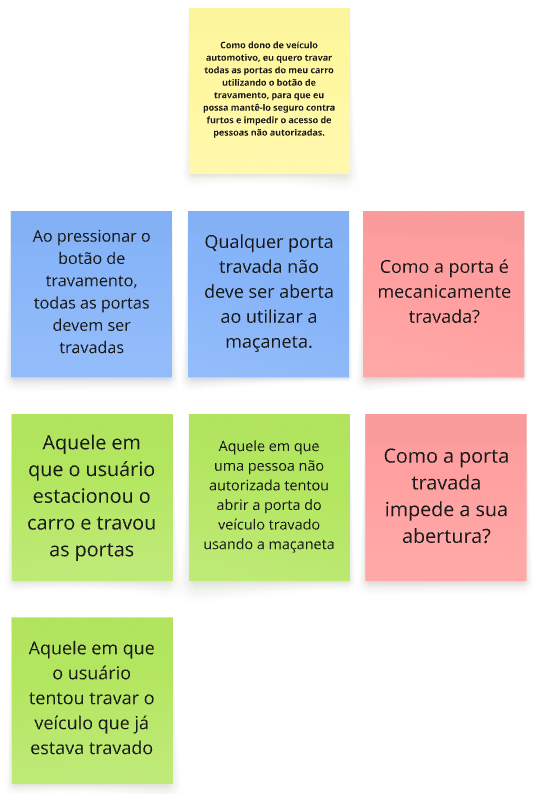
\includegraphics[height=12cm]{figuras/user_story_1.png}
\caption{História de Usuário 1: Travamento de todas as portas.}
\label{fig:historia1}
\end{figure}

Antes de seguir para a próxima história de usuário, aqui serão tratadas as perguntas que foram anotadas nesta seção. Esta etapa poderia ser postergada 
para o final do processo de discussão de exemplos, mas para garantir uma evolução incremental do produto, a próxima história será tratada quando os pontos 
abertos da atual forem respondidos.

Assim como descrito por \citeonline{reif2017locking}, sabe-se que existem 2 principais tipos de sistemas de travamento de porta que podem ser encontrados em veículos modernos:
\begin{itemize}
    \item Trava mecânica que é operada de maneira elétrica ou pneumática;
    \item Trava eletrônica que é montada com a trava e os eletrônicos embutidos.
\end{itemize}

Neste projeto, será implementado uma versão simulada de um sistema de trava eletrônica para se aproveitar de sua simplificação e menor número de componentes 
mecânicos no produto físico. Tipicamente, nesse sistema as maçanetas não precisam se mover ou podem até serem removidas inteiramente, podendo ser substituídas 
por botões equipados com sensores que se comunicam com a trava. Além disso, todos os componentes que transmitem o movimento da maçaneta no sistema mecânico aqui 
são desnecessários, substituídos pela fiação que se liga ao componente.

Embutido na trava eletrônica também é incluído o mecanismo básico de travamento como descrito por \citeonline{reif2017locking}. Ele é composto por três peças principais: 
o trinco (1) e engate (2) - que são acoplados à porta - e  o pino de batente (3) - que é acoplado ao chassi do veículo. Eles são responsáveis por manter a porta 
firmemente fechada, conforme ilustrado na figura 2:

\begin{figure}[H]
\centering
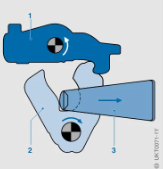
\includegraphics[height=6cm]{figuras/trava_mecanismo.png}
\caption{Mecanismo de travamento da porta. Fonte: \cite{reif2017locking}.}
\label{fig:travaporta}
\end{figure}

Durante o fechamento da porta, o engate (2) colide com o pino de batente (3) e gira no sentido anti-horário, passando por baixo do pino até retornar à sua posição 
inicial e fazer contato com o trinco (1). Nesse ponto, a trava encontra-se na posição fechada, exatamente como demonstrado na imagem, e qualquer tentativa de abrir 
a porta força o engate no sentido horário - movimento que é impedido pela presença do trinco.

Quando a porta está destravada, no entanto, é possível abri-la ao girar o trinco no sentido anti-horário. Esse movimento libera o engate, permitindo que ele se 
afaste do pino de batente e possibilite a abertura da porta.

No caso da trava eletrônica, o acionamento desse mecanismo é controlado por lógica implementada em software e transmitido por meio de um motor que é mecanicamente 
conectado ao trinco. Assim, respondendo à segunda pergunta, a porta trava se mantém fechada ao bloquear o movimento do trinco mediante o uso da maçaneta, da mesma 
forma que a abertura é feita ao mover o trinco.

Para modelar esse comportamento do sistema, o seu escopo pode ser definido em termos de lógica de aplicação e de software básico da seguinte maneira:

\begin{itemize}
    \item \textbf{Lógica de aplicação} - gera saídas em binário para cada porta, definindo se ela está travada ou destravada e se ela deve ser aberta ou mantida fechada;
    \item \textbf{Lógica de software básico} - recebe o sinal de saída em 0 ou 1 e o converte em sinais compreensíveis para o hardware de travamento, que resultam no movimento do motor.
\end{itemize}

Além do mecanismo de travamento em si, serão utilizados botões para realizar o travamento e abertura das portas. Seu escopo será feito de maneira similar, utilizando 
valores binários como abstrações dos sinais existentes a nível de hardware que são convertidos no software básico. Em suma, para atender a primeira história de 
usuário discutida, o modelo do sistema será desenvolvido tomando como base a lógica de aplicação assim como destacado na figura 3:

\begin{figure}[H]
\centering
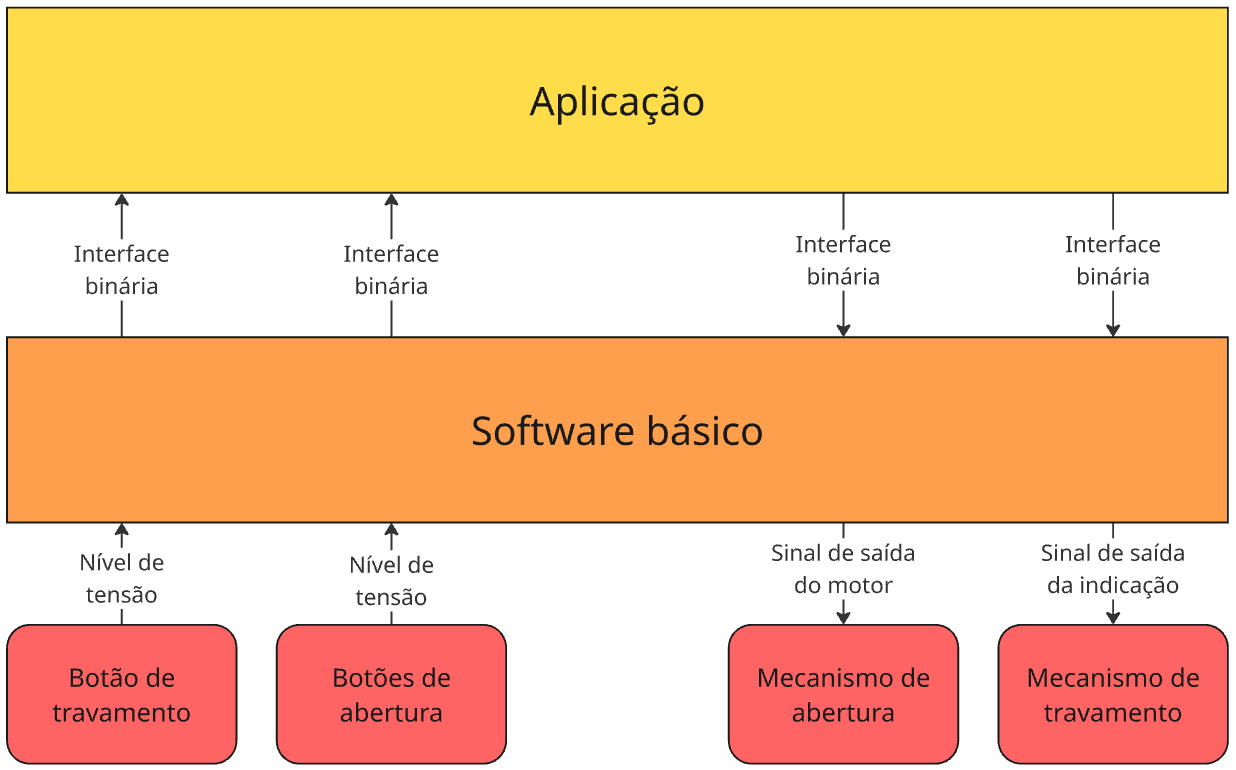
\includegraphics[height=8cm]{figuras/diagrama_aplication.png}
\caption{Diagrama de abstração do sistema em camadas de aplicação, software básico e componentes físicos.}
\label{fig:abstracaosw}
\end{figure}

Portanto, para a lógica de aplicação do modelo, receber o valor 1 recebido pela interface binária do botão de travamento é interpretado como um comando de 
pressionamento, da mesma forma que o valor 1 na interface do botão de abertura indica que a maçaneta foi acionada. No sentido oposto, ao enviar a saída para 
o software básico, esses valores são interpretados e convertidos em sinais de controle que determinam o movimento do motor.

Na prática, o travamento ou destravamento funciona apenas como uma limitação à abertura das portas e portanto, especialmente no caso da trava eletrônica, 
não há distinção física evidente entre os dois estados. Para facilitar essa identificação, este trabalho introduz uma indicação adicional, representada 
pelo ``Mecanismo de travamento'' na Figura \ref{fig:abstracaosw}. Ela servirá apenas para indicar o estado atual de cada porta, facilitando a execução dos 
testes e a validação funcional do sistema.

\subsection{História de usuário 2}
\label{sbs:historia2}

Ao considerar a história de usuário de destravamento das portas, é importante pensar na perspectiva da intenção de acessar o veículo. Isso é uma situação 
cotidiana que acontece com altíssima frequência, e portanto possui exemplos muito semelhantes a história 1:

\begin{itemize}
    \item \textbf{Aquele em que o usuário destravou as portas e entrou no carro} - situação típica de uso, ocorre sempre que o usuário retorna ao carro e precisa acessá-lo normalmente após o destravamento;
    \item \textbf{Aquele em que algumas portas já estavam destravadas} - caso em que o veículo se encontrava parcial ou totalmente destravado no momento em que o botão de destravamento foi acionado;
    \item \textbf{Aquele em que o usuário abriu a porta que estava destravada} -  situação em que, após o destravamento, o usuário acessa o veículo por meio da maçaneta, uma vez que a porta está destravada.
\end{itemize}

Para satisfazer os exemplos listados, as seguintes regras serão implementadas:

\begin{itemize}
    \item Ao pressionar o botão de destravamento, todas as portas devem ser destravadas.
    \item Qualquer porta destravada deve ser aberta ao utilizar a maçaneta.
\end{itemize}

Ao final, foram capturados 3 exemplos e 2 regras na história de usuário, o que compõe as seguintes notas coloridas:

\begin{figure}[H]
\centering
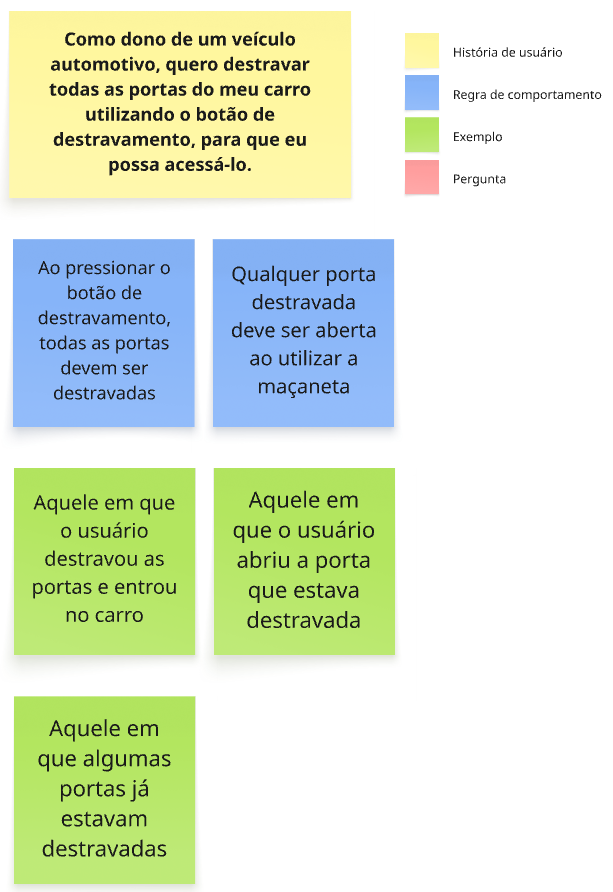
\includegraphics[height=12cm]{figuras/user_story_2.png}
\caption{História de Usuário 2: Destravamento de todas as portas.}
\label{fig:historia2}
\end{figure}

Com base nas respostas obtidas na história anterior, diversas incertezas acerca do funcionamento do destravamento das portas já foram determinadas. Sabe-se, 
por exemplo, que a porta destravada possui uma indicação de estado e que, ao pressionar o botão de abertura, a saída do modelo deve informar ao software básico 
que o mecanismo da porta deve ser liberado - ação que será realizada por meio do sinal de controle enviado ao motor.

A única distinção nesta história é a introdução de um novo botão: o botão de destravamento. Ele exige uma interface semelhante à descrita anteriormente, sendo 
igualmente interpretada pelo software básico como um valor de tensão e convertido em um sinal binário que indica o estado atual do botão.

\subsection{História de usuário 3}

A indicação da confirmação de travamento ou destravamento do veículo tem a grande importância de permitir que o usuário esteja assegurado de que o seu comando foi 
recebido e executado pelo veículo. Ela deve portanto ser invocada sempre que o usuário estiver utilizando as histórias 1 e 2, além de capturar 
os seguintes exemplos:

\begin{itemize}
    \item \textbf{Aquele em que o usuário travou seu veículo e ficou na dúvida se as portas foram travadas ou destravadas} - caso em que o usuário utiliza o botão de travamento e espera que o seu veículo seja assegurado. Deve invocar uma indicação distinta da indicação de destravamento;
    \item \textbf{Aquele em que o usuário destravou seu veículo e ficou na dúvida se as portas foram travadas ou destravadas} - caso em que o usuário utiliza o botão de destravamento e espera que o seu veículo seja destravado. Deve invocar uma indicação distinta da indicação de travamento;
    \item \textbf{Aquele em que o usuário tentou travar seu veículo sem perceber que uma das portas ficou aberta} - pode acontecer quando uma ou mais portas ficam abertas por conta de alguém esquecer de fechá-la. Neste caso, mesmo travando a porta que está aberta, o veículo ainda não fica seguro contra o acesso indevido e portanto deve invocar uma indicação de falha.
\end{itemize} 

O último exemplo destacado surgiu a partir de um questionamento levantado durante a idealização da história de usuário em análise. O objetivo é garantir que o usuário 
seja informado em situações nas quais, mesmo tendo solicitado o travamento das portas, o veículo ainda não possa ser devidamente assegurado devido à permanência de uma 
porta aberta.

Esse comportamento exige a emissão de um aviso distinto ao usuário, por meio de uma terceira forma de feedback que sinalize a condição de porta aberta. Dessa maneira, 
assegura-se que o valor identificado seja atendido, especialmente considerando que, conforme definido na primeira história, o acionamento do botão de travamento expressa 
a intenção do usuário de proteger o veículo.

As regras que cobrem os exemplos listados são:

\begin{itemize}
    \item O veículo deve indicar que foi travado ou destravado com sucesso utilizando sinais distintos para cada comando;
    \item O veículo deve indicar com um sinal de falha quando pelo menos uma das portas está aberta ao receber o comando de travamento.
\end{itemize}

O último exemplo levanta questões que precisam ser exploradas por meio de perguntas e trazem consigo um novo fator que o sistema deve considerar: o estado de 
abertura das portas. Para isso, as seguintes perguntas são criadas:

\begin{itemize}
    \item Como o sistema detecta se uma porta está aberta ou fechada?
    \item É possível travar ou destravar uma porta que está aberta?
\end{itemize}

Dessa forma, essa história de usuário foi mapeada com 3 exemplos, 2 regras e 2 perguntas, de acordo com a Figura \ref{fig:historia3}:

\begin{figure}[H]
\centering
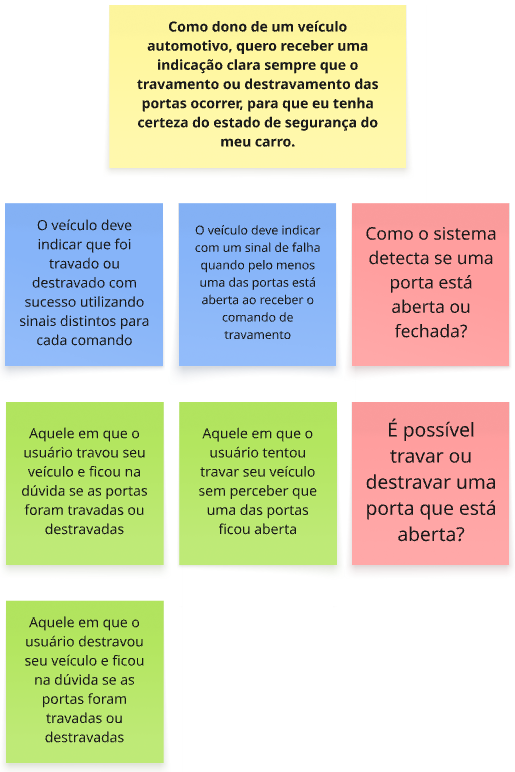
\includegraphics[height=12cm]{figuras/user_story_3.png}
\caption{História de Usuário 3: Feedback de travamento.}
\label{fig:historia3}
\end{figure}

A investigação das perguntas levantadas envolvem detalhes que dependem diretamente da implementação física do produto. Para respondê-las, é necessário 
compreender como um sistema veicular real consegue identificar se as portas estão fisicamente abertas.

Esta detecção é normalmente feita por meio de sensores ou mecanismos capazes de indicar quando a porta está entreaberta (estado \textit{ajar}). Um exemplo é 
apresentado em \citeonline{us4566285a}, que descreve o uso de switches físicos: eles são pressionados quando a porta está completamente fechada e liberados 
quando a porta se abre. 

Esse tipo de sensor pode ser integrado de forma semelhante às interfaces binárias utilizadas nos botões de travamento e destravamento, empregando sinais 
binários (0 ou 1) para representar os estados ``fechada'' ou ``aberta'' da porta. Com essa informação, o sistema pode combinar o estado físico da porta com a 
entrada da interface do botão de travamento para determinar quando o alerta para o usuário deve ser realizado.

É importante destacar que, embora o controle de abertura da porta seja gerenciado pelo sistema, a utilização de um sensor continua sendo essencial para 
determinar seu estado real. Esse cenário é comum no controle de componentes mecânicos, em que parte do comportamento não é governada diretamente pela 
lógica de software ou eletrônica.

No caso em questão, a saída final do sistema de travamento consiste no acionamento do motor que movimenta o trinco e libera o mecanismo da trava, permitindo 
que a porta seja aberta. No entanto, uma vez que essa ação é executada, o sistema não tem como saber se o usuário realmente abriu a porta - ou se, após abri-la, 
voltou a fechá-la - sem o auxílio de um sensor. Isso ocorre porque a abertura da porta é uma ação mecânica realizada pelo usuário, sendo apenas condicionada, e 
não diretamente executada, pelo sistema eletrônico em desenvolvimento.

Além disso, o travamento e destravamento das portas é realizado de maneira independente do estado da porta e pode ser realizado mesmo que ela esteja aberta. Isso 
deve-se ao fato de que o controlador eletrônico é responsável por definir quando o mecanismo da trava deve ser acionado. Caso a porta esteja destravada, esta ação 
é tomada após o pressionar do botão de abertura da porta.

Em termos práticos, isso significa que não existe diferença física entre uma porta travada ou destravada, este é apenas um estado que é virtualmente definido 
pelo controlador. É importante ressaltar que travar uma porta aberta ainda não satisfaz a condição de assegurar o veículo, como definido na primeira história 
de usuário e por conta disso o alerta do usuário se vê necessário.

\subsection{História de usuário 4}

A funcionalidade de \textit{Keyless Access} permite o destravamento individual das portas assim que o usuário aciona a maçaneta de uma porta travada, desde que a chave 
autorizada esteja presente em sua posse. Os exemplos de uso dessa funcionalidade são bastante semelhantes aos do destravamento convencional, pois refletem 
situações em que o usuário tem a intenção de acessar o veículo. 

Neste estágio, ainda não foi definida a tecnologia que será utilizada para a identificação da chave. Por isso, essa incerteza será tratada por meio de uma 
pergunta associada a esta história de usuário.

Os exemplos capturados na discussão da história são:

\begin{itemize}
    \item \textbf{Aquele em que o usuário tinha a chave no bolso e usou a maçaneta} - Este é o caso típico de uso da funcionalidade: a chave autorizada está próxima e é reconhecida pelo sistema, permitindo o destravamento imediato da porta acionada;
    \item \textbf{Aquele em que outra pessoa abriu outra porta simultaneamente} - Neste caso, mais uma porta é aberta simultaneamente, possivelmente por alguém acompanhando o dono do veículo. O sistema deve tratar as portas de forma independente, e portanto ambas devem ser destravadas individualmente, permitindo o acesso simultâneo;
    \item \textbf{Aquele em que o usuário destravou a porta e a fechou de novo} - Após acessar o veículo utilizando o \textit{Keyless Access} e em seguida fechar a porta, o sistema deve manter a porta destravada até que o usuário execute explicitamente o comando de travamento. Isso garante que a intenção do usuário seja respeitada e evita travamentos não intencionais.
\end{itemize}

Para cobrir os exemplos, as seguintes regras serão utilizadas:

\begin{itemize}
    \item Qualquer porta que tiver sua maçaneta utilizada deve ser destravada desde que a chave esteja próxima ao veículo;
    \item A porta deve ser mantida destravada após a operação de \textit{Keyless Access}.
\end{itemize}

O mapeamento de exemplos dessa história na forma de notas coloridas é composto por 3 exemplos, 2 regras e 1 pergunta:

\begin{figure}[H]
\centering
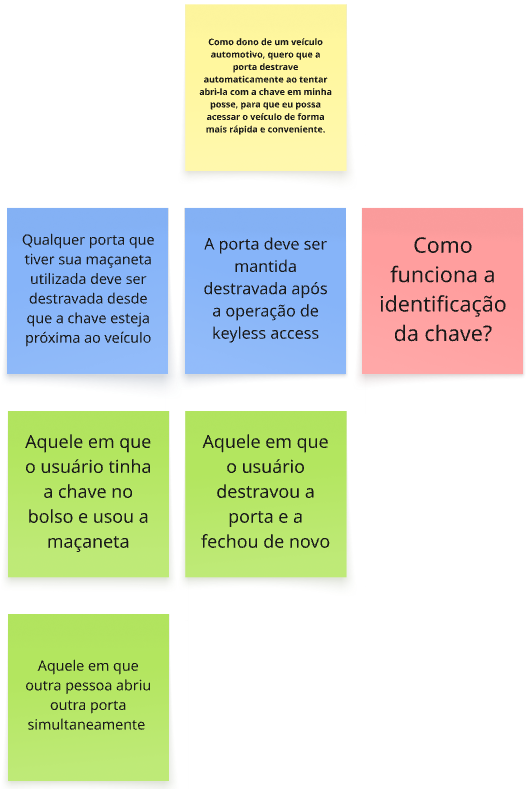
\includegraphics[height=12cm]{figuras/user_story_4.png}
\caption{História de Usuário 4: \textit{Keyless Access}.}
\label{fig:historia4}
\end{figure}

Por fim, uma nova pergunta foi levantada no mapeamento de exemplos da história e deve ser respondida antes do trabalho na próxima história. Para fazê-lo, é 
preciso investigar alguma opção de tecnologia que possa ser utilizada para representar a validação de chave de usuário. 

A implementação de sistemas de detecção de chave, conforme descrito por \citeonline{glocker2016protocol}, costumam utilizar módulos de comunicação por rádio-frequência (RF), 
capazes de estabelecer conexão com um dispositivo autorizado. A validação desse dispositivo pode ser realizada por meio de diferentes métodos e protocolos de segurança, 
que incluem mecanismos de autenticação mútua entre a chave e o veículo. Esses protocolos aumentam a robustez do sistema contra tentativas de acesso não autorizado.

Em casos mais simples, como demonstrado em \citeonline{arduinoRFID}, o sistema utiliza um sensor \textit{RFID (Radio Frequency Identification)} e uma tag que contém uma chave 
de identificação única. O funcionamento baseia-se na transmissão do identificador por meio de um sinal de rádio quando a tag é aproximada do sensor. O sensor, 
por sua vez, envia o código recebido ao microcontrolador, que o compara com um identificador previamente armazenado em sua memória. Caso haja correspondência, 
a chave é considerada válida e o acesso é autorizado.

Esse tipo de autenticação, no contexto da arquitetura \textit{AUTOSAR}, é normalmente responsabilidade de um componente específico do software básico pertencente 
à pilha de cibersegurança. Esse componente, conhecido como \textit{Key Manager} \cite{autosarKeyManager}, fornece serviços utilizados para a validação de chaves, 
utilizando diferentes protocolos de segurança. Ele também se comunica com a unidade de memória do controlador para acessar os dados das chaves previamente registradas.

Considerando a presença desse componente no sistema \textit{AUTOSAR}, será adotada novamente uma abstração da tecnologia de hardware envolvida, por meio de uma interface 
binária. Nesse cenário, a verificação da chave de identificação em relação ao valor armazenado em memória é realizada pelo \textit{Key Manager} e o resultado dessa 
validação é então comunicado à aplicação de forma semelhante ao funcionamento dos botões de entrada: por meio de um sinal binário que indica se a chave foi 
validada (1) ou não (0).

\subsection{História de usuário 5}
A funcionalidade de auto travamento é comumente implementada para contemplar diferentes cenários de uso do veículo. Neste caso específico, o foco está na situação em 
que as portas são destravadas de forma não intencional. Antes de apresentar os exemplos, será feita uma definição do que se entende por ``não intenção'' por parte do 
usuário, considerando que, na prática, essa intenção precisa ser inferida com base nas entradas disponíveis no sistema. 

Esse tipo de questão costuma ser capturado em perguntas, nas notas vermelhas, para que possa ser investigado após o mapeamento de exemplos. No entanto, para essa 
história é essencial que a definição de não intencional seja feita, pois ela definirá com clareza que exemplos de uso devem ser mapeados.

De modo geral, o destravamento das portas tem como objetivo permitir o acesso ao veículo, o que se concretiza quando o usuário abre pelo menos uma das portas. Utilizando 
esse critério, a ausência da abertura das portas dentro de um determinado intervalo de tempo após o destravamento pode ser interpretada como um indicativo de que o 
usuário não teve a intenção consciente de destravar o veículo. 

Essa condição também é presente em veículos Volkswagen, assim como descrito no manual do usuário \cite{vwLocking}. Segundo ele, o veículo realiza o travamento automático 
em até 45 segundos após ter sido destravado, desde que, entre outras possíveis condições, nenhuma das portas tenha sido aberta. A fim de tornar a ação de travamento 
automático mais rápida e facilitar a execução dos testes, o tempo de espera para essa condição será reduzido para 15 segundos neste trabalho.

Adicionalmente, o estado inicial das portas no momento do destravamento também é de relevância para esse comportamento. Nos casos em que o veículo não estava 
completamente travado previamente, infere-se que o usuário não possuía a intenção de garantir a segurança do veículo, mesmo antes do botão de destravamento ser 
pressionado, e portanto ele não precisa ser travado novamente.

Sabe-se que o principal objetivo do travamento do veículo é garantir sua segurança contra furtos e impedir o acesso de pessoas não autorizadas. No entanto, existem 
cenários em que o usuário pode intencionalmente optar por deixar o veículo destravado, mesmo que não pretenda acessá-lo de imediato. Um exemplo disso seria quando 
o veículo é deixado em uma garagem particular, onde o usuário deseja mantê-lo acessível para buscar um item posteriormente ou por qualquer outro motivo, sem a 
necessidade de utilizar novamente a chave ou o sistema de \textit{Keyless Access}.

Para contemplar essa situação e permitir que a intenção do usuário seja respeitada, é necessário que exista pelo menos uma regra específica que permita o 
destravamento completo, sem que seja necessário o acesso ao veículo. Neste caso, será adotada a estratégia de considerar o duplo acionamento do botão de 
destravamento como uma indicação explícita da intenção de manter o veículo destravado. 

Por fim, os exemplos capturados na história são:

\begin{itemize}
    \item \textbf{Aquele em que o usuário destravou mas não foi acessar o carro} - este é o cenário padrão de destravamento não intencional, que pode ocorrer por diversos motivos, como o acionamento acidental do botão de destravamento. Nessa situação, o sistema realizará o travamento automático após um intervalo de tempo pré-definido, interpretando que não houve intenção de acesso;
    \item \textbf{Aquele em que o usuário destravou e foi acessar o carro} - neste cenário, a situação oposta à do exemplo anterior acontece, pois o usuário acessou o veículo, abrindo uma das portas, em tempo. O travamento automático não deve ser acionado neste caso;
    \item \textbf{Aquele em que o usuário pressionou o botão de destravamento duas vezes para manter o carro destravado} - Quando for da intenção do usuário deixar o veículo destravado sem abrir nenhuma porta, a função de travamento automático será inibida mediante o duplo acionamento do botão de destravamento. Essa ação será interpretada como uma indicação explícita da intenção de manter o veículo acessível;
    \item \textbf{Aquele em que o usuário destravou o veículo quando ele já estava acessível} - refere-se às situações em que o veículo não estava completamente travado inicialmente, seja porque uma ou mais portas já estavam destravadas ou por conta do acionamento repetido do botão de destravamento. Nestes casos, o sistema entende que o usuário já interagiu com o veículo e portanto o travamento automático também não será executado.
\end{itemize}

Com os exemplos mapeados, o comportamento definido garante que o travamento automático trata em específico os casos em que a ação do usuário indicou que ele não possuía a intenção de mudar o veículo de um estado inicial em que ele está absolutamente seguro contra furtos - todas as portas estavam travadas - para o caso em que qualquer pessoa poderia acessá-lo. As regras que satisfazem os exemplos são:

\begin{itemize}
    \item Travar automaticamente caso o botão de destravamento seja usado uma vez e nenhuma porta seja aberta;
    \item Não travar caso o botão de destravamento seja pressionado uma segunda vez;
    \item Não travar caso o veículo não esteja completamente travado antes do destravamento.
\end{itemize}

O mapeamento de exemplos dessa história na forma de notas coloridas é composto por 4 exemplos e 3 regras:

\begin{figure}[H]
\centering
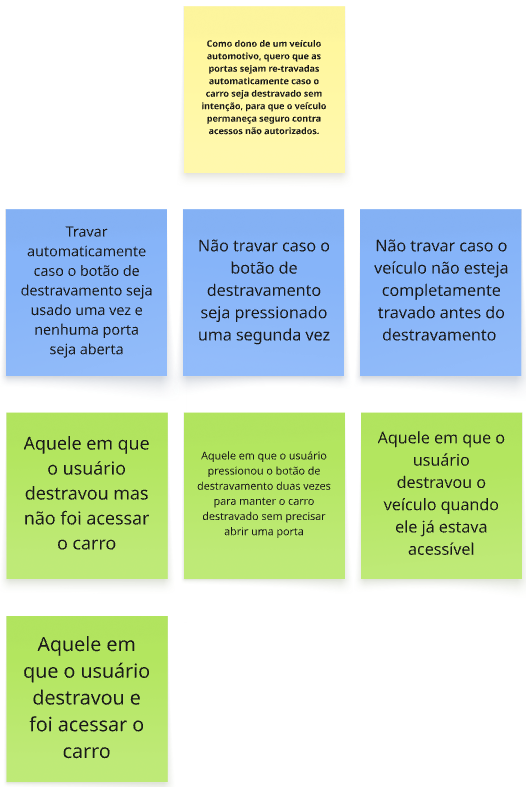
\includegraphics[height=12cm]{figuras/user_story_5.png}
\caption{História de Usuário 5: Travamento automático.}
\label{fig:historia5}
\end{figure}

\section{\textbf{Etapa 3: Desenho do diagrama de caixa preta}}
\label{sbs:etapa3}
Com todas as histórias de usuário definidas, o próximo passo do trabalho consiste na elaboração do diagrama de caixa preta, com o objetivo de identificar todas as 
interfaces necessárias para suportar os comportamentos previamente levantados. Essa etapa é essencial para garantir que todas as interações entre o usuário e o 
sistema estejam claramente especificadas e para suportar a criação dos cenários \textit{Gherkin} a seguir.

Para dar início ao processo, é necessário listar todas as entradas e saídas do sistema:

\textbf{Entradas}:

\begin{itemize}
    \item Botão de travamento
    \item Botão de destravamento
    \item Botões de abertura das portas (4 no total)
    \item Sensores de abertura das portas (4 no total)
    \item Detecção de chave autenticada.
\end{itemize}

\textbf{Saídas}:

\begin{itemize}
    \item Indicação de estado de travamento de todas as portas (4 no total)
    \item Estado da tranca de cada porta (4 no total)
    \item Feedback para o usuário.
\end{itemize}

O diagrama é então elaborado com um bloco central representando o sistema, ao qual estão conectadas todas as interfaces previamente listadas. Neste estágio, 
o bloco central permanece sem conteúdo interno, uma vez que o objetivo é abstrair os detalhes da implementação e focar exclusivamente na definição das 
interações entre o sistema e o usuário.

Dessa forma, o diagrama assume a configuração ilustrada na Figura \ref{fig:caixapreta}:

\begin{figure}[H]
\centering
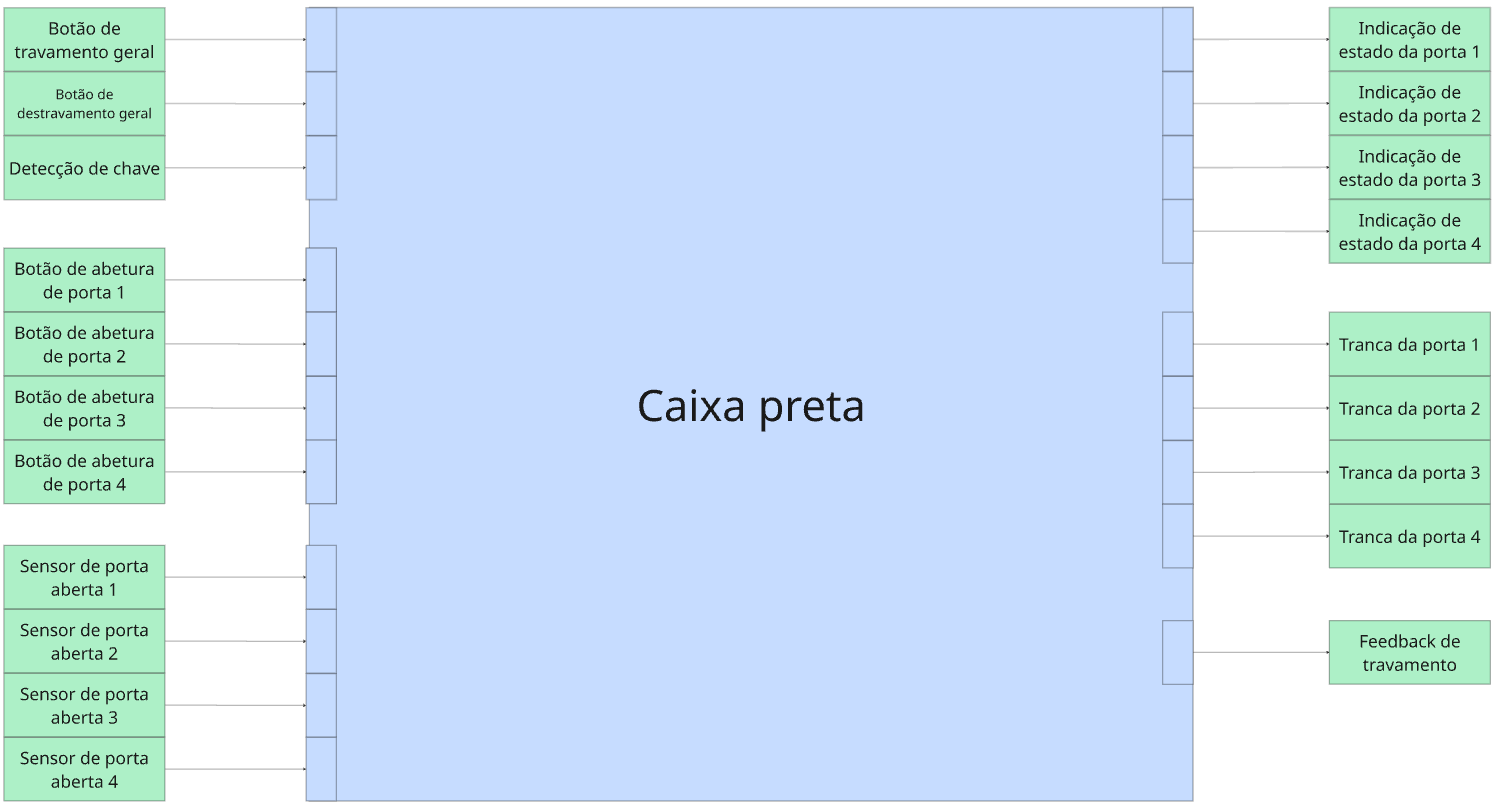
\includegraphics[height=8cm]{figuras/diagrama_caixa_preta.png}
\caption{Diagrama de Caixa Preta do sistema de travamento de portas.}
\label{fig:caixapreta}
\end{figure}

De maneira análoga, o modelo desenvolvido no Simulink também deverá adotar uma estrutura semelhante, composta por um modelo de alto nível - que define apenas as 
entradas e saídas do sistema - e um modelo de baixo nível, responsável por conter toda a lógica funcional implementada.

É importante destacar que algumas interfaces adicionais serão necessárias no modelo do sistema, embora não estejam representadas no diagrama de caixa preta, 
pois não estão diretamente relacionadas aos comportamentos observáveis pelo usuário. Essas interfaces serão detalhadas no Capítulo \ref{ch:RD}, e são fundamentais para suportar aspectos técnicos que garantem o funcionamento correto do sistema. Um exemplo dessas interfaces é o tempo 
de simulação, necessário para validar a condição de auto travamento descrita na história de usuário 5.

Para finalizar essa etapa, é necessário definir quais são os valores possíveis que devem ser capturados em cada uma das interfaces criadas no diagrama da Figura \ref{fig:caixapreta}.

% \begin{tabular}{|p{5cm}|p{7cm}|}
% %\centering
% %\caption{Valores possíveis para as interfaces de entrada e saída}
% %\addcontentsline{loq}{table}{\protect\numberline{\thetable}Valores possíveis para as interfaces de entrada e saída}
% \hline
% Nome da interface 1 & Valores Possíveis \\ 
% \hline
% Botão de travamento geral & 
% \begin{itemize}[topsep=0pt, partopsep=0pt, leftmargin=*]
%     \item Pressionado
%     \item Solto
% \end{itemize} \\
% \hline
% Botão de destravamento geral &
% \begin{itemize}[topsep=0pt, partopsep=0pt, leftmargin=*]
%     \item Pressionado
%     \item Solto
% \end{itemize} \\
% \hline
% Detecção de chave &
% \begin{itemize}[topsep=0pt, partopsep=0pt, leftmargin=*]
%     \item Presente
%     \item Não presente
% \end{itemize} \\
% \hline
% Botão de abetura de porta (de 1 a 4) &
% \begin{itemize}[topsep=0pt, partopsep=0pt, leftmargin=*]
%     \item Pressionado
%     \item Solto
% \end{itemize} \\
% \hline
% Sensor de porta aberta (de 1 a 4) &
% \begin{itemize}[topsep=0pt, partopsep=0pt, leftmargin=*]
%     \item Fechada
%     \item Aberta
% \end{itemize} \\
% \hline
% Indicação de estado da porta (de 1 a 4) &
% \begin{itemize}[topsep=0pt, partopsep=0pt, leftmargin=*]
%     \item Travada
%     \item Destravada
% \end{itemize} \\
% \hline
% Tranca da porta 1 &
% \begin{itemize}[topsep=0pt, partopsep=0pt, leftmargin=*]
%     \item Segura
%     \item Solta
% \end{itemize} \\
% \hline
% Feedback de travamento &
% \begin{itemize}[topsep=0pt, partopsep=0pt, leftmargin=*]
%     \item Confirmação de trava
%     \item Confirmação de destrava
%     \item Operação falha
% \end{itemize} \\
% \hline
% %\label{qua:interfaces}
% \end{tabular}

\begin{quadro}[h]
\caption{Valores possíveis para as interfaces de entrada e saída}
\label{qua:interfaces}
\begin{tabular}{|p{5cm}|p{7cm}|}
\hline
Nome da interface 1 & Valores Possíveis \\ 
\hline
Botão de travamento geral & 
\begin{itemize}[topsep=0pt, partopsep=0pt, leftmargin=*]
    \item Pressionado
    \item Solto
\end{itemize} \\
\hline
Botão de destravamento geral &
\begin{itemize}[topsep=0pt, partopsep=0pt, leftmargin=*]
    \item Pressionado
    \item Solto
\end{itemize} \\
\hline
Detecção de chave &
\begin{itemize}[topsep=0pt, partopsep=0pt, leftmargin=*]
    \item Presente
    \item Não presente
\end{itemize} \\
\hline
Botão de abertura de porta (de 1 a 4) &
\begin{itemize}[topsep=0pt, partopsep=0pt, leftmargin=*]
    \item Pressionado
    \item Solto
\end{itemize} \\
\hline
Sensor de porta aberta (de 1 a 4) &
\begin{itemize}[topsep=0pt, partopsep=0pt, leftmargin=*]
    \item Fechada
    \item Aberta
\end{itemize} \\
\hline
Indicação de estado da porta (de 1 a 4) &
\begin{itemize}[topsep=0pt, partopsep=0pt, leftmargin=*]
    \item Travada
    \item Destravada
\end{itemize} \\
\hline
Tranca da porta 1 &
\begin{itemize}[topsep=0pt, partopsep=0pt, leftmargin=*]
    \item Segura
    \item Solta
\end{itemize} \\
\hline
Feedback de travamento &
\begin{itemize}[topsep=0pt, partopsep=0pt, leftmargin=*]
    \item Sem status
    \item Confirmação de trava
    \item Confirmação de destrava
    \item Operação falha
\end{itemize} \\
\hline
\end{tabular}
\end{quadro}

Neste quadro, os valores das interfaces foram descritos de maneira textual, com valores que se aplicam à linguagem natural proposta pela metodologia de BDD. 
Na prática, todos os valores serão utilizados como enumerações convertidas para um valor numérico que representa o estado da interface.

\section{\textbf{Etapa 4: Desenvolvimento dos cenários Gherkin}}
\label{sbs:etapa4}
Nesta etapa, os cenários \textit{Gherkin} serão desenvolvidos e utilizados como critérios de aceitação das histórias previamente definidas. Estes cenários devem ser capazes 
de cobrir todos os exemplos capturados durante o mapeamento, assegurando que o desenvolvimento do sistema atenda à experiência de usuário desejada.
Como primeiro passo, será definida a estrutura de pastas do projeto, responsável por organizar tanto os arquivos \texttt{.feature} - um para cada história de usuário - 
quanto o modelo em Simulink. Seguindo a estrutura recomendada na documentação da biblioteca Behave \cite{behaveDocs}, o projeto será organizado da seguinte forma hierárquica:

\begin{verbatim}
    projeto/
    |-- features/
    |   |-- lock\_all.feature
    |   |-- unlock\_all.feature
    |   |-- locking\_feedback.feature
    |   |-- unlock\_individual.feature
    |   |-- auto\_relock.feature
    |   `-- steps/
    |       `-- lock\_unlock.py
\end{verbatim}

Cada história de usuário possui um arquivo \texttt{\.feature} correspondente, todos organizados dentro da pasta \texttt{features} do projeto. A nomenclatura desses 
arquivos foi definida de forma a evidenciar a funcionalidade representada em cada um, facilitando a identificação e o rastreamento das histórias implementadas. 
Por exemplo, o arquivo \texttt{lock\_all.feature} refere-se à primeira história de usuário, que descreve a funcionalidade de travamento de todas as portas 
por meio do botão de travamento.

Além disso, o arquivo environment.py é utilizado para definir funções de inicialização que são executadas antes do início dos testes ou de cada passo individual. 
Uma de suas responsabilidades é iniciar a simulação quando os testes são acionados, além de disponibilizar interfaces que permitem a comunicação com o modelo Simulink.

Por fim, o arquivo de definição dos passos \textit{(step definitions)} é armazenado na pasta steps e foi nomeado de \texttt{lock\_unlock.py}. Ele é responsável por mapear os 
passos descritos nos cenários \textit{Gherkin} para funções executáveis, que realizam as ações esperadas e interagem com o modelo.

É importante destacar que o desenvolvimento dos cenários \textit{Gherkin} é um processo iterativo, que deve evoluir de acordo com o grau de maturidade do sistema. 
Por esse motivo, como será demonstrado na etapa de modelagem, ajustes pontuais nos cenários - como a adição de passos que facilitem a execução da simulação - 
poderão ser realizados ao longo do tempo.

Durante a criação dos cenários, alguns cuidados serão adotados para garantir consistência e reutilização. Um desses cuidados é a definição de passos genéricos 
e reutilizáveis, especialmente para ações recorrentes. Por exemplo, nas histórias 1 e 5, que descrevem funcionalidades que resultam no travamento completo do 
veículo, é possível validar o estado final utilizando um mesmo passo compartilhado, como \texttt{Then todas as portas deveriam estar travadas}.

Uma possível definição para esse passo consiste em realizar a leitura dos valores presentes nas quatro interfaces de saída do modelo, que indicam o estado atual 
de cada porta. Considerando que o valor 1 representa uma porta travada, a função deve verificar se todas as saídas possuem esse valor, aprovando o teste apenas se 
essa condição for satisfeita.

Para torná-la ainda mais reutilizável, essa função pode incorporar um parâmetro textual extraído diretamente do passo \textit{Gherkin}, permitindo que parte da frase do 
cenário seja utilizada como argumento. Dessa forma, a lógica de verificação pode ser adaptada dinamicamente: por exemplo, a função pode identificar se a última 
palavra do passo é ``travadas'' ou ``destravadas'' e, com base nisso, validar se os valores lidos são 1 (para travadas) ou 0 (para destravadas), aprovando o teste 
conforme o caso.

Outra funcionalidade importante empregada na escrita dos cenários é o uso de tabelas de exemplos \textit{(Examples)}, que possibilitam a execução repetida de um mesmo 
cenário com diferentes combinações de parâmetros. Essa abordagem é especialmente útil para validar comportamentos sob múltiplas condições iniciais, evitando a 
necessidade de duplicar cenários com estruturas idênticas.

Por exemplo, a primeira história de usuário define que, ao pressionar o botão de travamento, todas as portas devem ser travadas, independentemente de seu estado 
inicial. Para verificar esse comportamento, é possível parametrizar o estado de cada porta utilizando a cláusula Given combinada com a tabela de exemplos, 
como mostrado abaixo:

\begin{verbatim}
    Given a porta 1 está <estado1>
    
    Examples:
    | estado1    |
    | travada    |
    | destravada |
\end{verbatim}


Ao utilizar a sintaxe \texttt{<...>}, o Behave interpreta o conteúdo como uma variável, cujo valor será substituído com base nas linhas da tabela Examples. Cada 
linha da tabela gera um cenário independente, preservando a estrutura original, mas substituindo os parâmetros pelos respectivos valores.

Dessa forma, durante a execução, o Behave processa o cenário duas vezes. Na primeira execução, o passo é \texttt{Given a porta 1 está travada} e na segunda 
ele é \texttt{Given a porta 1 está destravada}.

Essa estrutura oferece grande flexibilidade na criação dos cenários e assegura a cobertura completa das possíveis combinações. No cenário real que será apresentado 
a seguir, existem 16 combinações possíveis, resultantes dos diferentes estados (travada ou destravada) das quatro portas.

Por fim, a funcionalidade \textit{Background} também será utilizada nos arquivos .feature para definir um estado inicial comum a todos os cenários. Essa estrutura permite 
declarar uma sequência de passos Given que serão executados automaticamente antes de cada cenário presente no arquivo. Isso evita a repetição de passos que se 
aplicam a múltiplos cenários, promovendo maior clareza e reutilização na especificação dos testes.

\subsection{História de usuário 1}

Uma maneira eficaz de estruturar o cenário \textit{Gherkin} é adotar a perspectiva do usuário e tentar descrever o comportamento esperado como uma sequência de ações, 
utilizando as cláusulas Given, When e Then. Tomando como base o primeiro exemplo da história - ``aquele em que o usuário estacionou o carro e travou as portas'' - 
o cenário pode ser representado da seguinte forma:

\begin{verbatim}
    Given o carro estava destravado ao ser estacionado
    When o usuário pressionou o botão de travamento
    Then todas as portas foram travadas
\end{verbatim}

Além disso, é possível aplicar o recurso de tabelas de exemplos \textit{(Examples)} para generalizar o cenário e incluir o segundo exemplo descrito na história: ``aquele 
em que o usuário tentou travar o veículo que já estava travado''. Nesse caso, substitui-se a primeira condição \textit{(Given)} por um conjunto de passos que definem 
individualmente o estado inicial de cada porta, utilizando os valores fornecidos pela tabela para simular todas as combinações possíveis de estados iniciais. 
A resposta final do sistema é comum entre os exemplos já que ambos compartilham o mesmo resultado final - a mesma cláusula \textit{Then}. 

Dessa forma, o primeiro exemplo é coberto em uma das linhas da tabela - a que define que todas as portas estão inicialmente destravadas - e o segundo é coberto 
por todas as demais linhas - que definem todas as possíveis combinações de estado para cada porta. O cenário geral pode assumir a seguinte forma:

\begin{verbatim}
Scenario Outline: Locking all doors
    Given the door '1' is <door_1_state>
    And the door '2' is <door_2_state>
    And the door '3' is <door_3_state>
    And the door '4' is <door_4_state>

    When I press the vehicle 'lock' button
    Then all doors should be 'locked'

    Examples:
        | door_1_state | door_2_state | door_3_state | door_4_state |
        | unlocked     | unlocked     | unlocked     | unlocked     |
        | unlocked     | unlocked     | unlocked     | locked       |
        | unlocked     | unlocked     | locked       | unlocked     |
        | unlocked     | unlocked     | locked       | locked       |
        | unlocked     | locked       | unlocked     | unlocked     |
        | unlocked     | locked       | unlocked     | locked       |
        | unlocked     | locked       | locked       | unlocked     |
        | unlocked     | locked       | locked       | locked       |
        | locked       | unlocked     | unlocked     | unlocked     |
        | locked       | unlocked     | unlocked     | locked       |
        | locked       | unlocked     | locked       | unlocked     |
        | locked       | unlocked     | locked       | locked       |
        | locked       | locked       | unlocked     | unlocked     |
        | locked       | locked       | unlocked     | locked       |
        | locked       | locked       | locked       | unlocked     |
        | locked       | locked       | locked       | locked       |
\end{verbatim}

A cláusula \textit{Given} utiliza quatro passos para definir os valores iniciais de cada porta, de forma que cada um recebe uma variável correspondente a uma coluna da 
tabela de exemplos. Essa tabela contém 16 linhas, que representam todas as combinações possíveis entre os estados ``travada'' e ``destravada'' para as quatro portas.

Na cláusula \textit{When}, é descrita a ação do usuário ao pressionar o botão de travamento. Em seguida, a cláusula \textit{Then} especifica que todas as portas devem estar travadas, 
validando assim o comportamento esperado de assegurar o veículo independentemente de seu estado inicial.

O último exemplo a ser coberto é: ``aquele em que uma pessoa não autorizada tentou abrir a porta do veículo travado usando a maçaneta''. Ele é validado por um 
cenário em que a porta continua fechada após a o botão de abertura ser pressionado, tendo em vista que ela está travada.

Para evitar a duplicação de cenários, a tabela de exemplos é novamente utilizada, permitindo a execução automática do teste para cada porta individualmente, variando 
apenas o ponto de interação. Ao final, o cenário assume a seguinte forma:

\begin{verbatim}

    Scenario Outline: Door cannot be released when locked
        Given the door <door_id> is 'locked'
        When I 'press' the door <door_id> release button
        Then the door <door_id> should be 'held'

        Examples:
            | door_id |
            | 1       |
            | 2       |
            | 3       |
            | 4       |

\end{verbatim}


\subsection{História de usuário 2}

A segunda história de usuário tem grande semelhança com a primeira e possui exemplos mapeados com casos de uso que são análogos à de travamento das portas. O 
primeiro cenário criado para esta história é:

\begin{verbatim}
Scenario Outline: Unlocking all doors    
    Given the door '1' is <door_1_state>
    And the door '2' is <door_2_state>
    And the door '3' is <door_3_state>
    And the door '4' is <door_4_state>

    When I press the vehicle 'unlock' button
    Then all doors should be 'unlocked'

    Examples:
        | door_1_state  | door_2_state  | door_3_state  | door_4_state  |
        | unlocked      | unlocked      | unlocked      | unlocked      |
        | unlocked      | unlocked      | unlocked      | locked        |
        | unlocked      | unlocked      | locked        | unlocked      |
        | unlocked      | unlocked      | locked        | locked        |
        | unlocked      | locked        | unlocked      | unlocked      |
        | unlocked      | locked        | unlocked      | locked        |
        | unlocked      | locked        | locked        | unlocked      |
        | unlocked      | locked        | locked        | locked        |
        | locked        | unlocked      | unlocked      | unlocked      |
        | locked        | unlocked      | unlocked      | locked        |
        | locked        | unlocked      | locked        | unlocked      |
        | locked        | unlocked      | locked        | locked        |
        | locked        | locked        | unlocked      | unlocked      |
        | locked        | locked        | unlocked      | locked        |
        | locked        | locked        | locked        | unlocked      |
        | locked        | locked        | locked        | locked        |
\end{verbatim}

Este cenário define que, com as pré-condições que cobrem todas as possíveis combinações de travamento e destravamento para cada porta, após o botão de destravamento 
ser pressionado, o veículo será destravado. Ele cobre os dois primeiros exemplos mapeados:
\begin{itemize}
    \item Aquele em que o usuário destravou as portas e entrou no carro;
    \item Aquele em que algumas portas já estavam destravadas.
\end{itemize}

Para o último exemplo, o seguinte cenário será utilizado:

\begin{verbatim}
    Scenario Outline: Door can be released when unlocked
        Given the door <door_id> is 'unlocked'
        When I 'press' the door <door_id> release button
        Then the door <door_id> should be 'released'

        Examples:
            | door_id |
            | 1       |
            | 2       |
            | 3       |
            | 4       |
\end{verbatim}

Este cenário, que é executado para cada uma das portas, define que a porta será aberta após o botão de abertura ser pressionado, tendo em vista que ela 
está destravada. Ele cobre o seguinte exemplo mapeado:

\begin{itemize}
    \item Aquele em que o usuário abriu a porta que estava destravada.
\end{itemize}


\subsection{História de usuário 3}

Para especificar o comportamento descrito nesta história, é necessário criar um novo tipo de passo que valide qual resposta de feedback foi acionada pelo veículo. 
Isso pode ser feito de acordo com o cenário:

\begin{verbatim}
Scenario Outline: Locking feedback when locking or unlocking the vehicle
    When I press the vehicle <operation> button

    Then all doors should be <state>
    And I should receive a <feedback> feedback

    Examples:
        | operation | state    | feedback               |
        | lock      | locked   | locking confirmation   |
        | unlock    | unlocked | unlocking confirmation |
\end{verbatim}

Esse cenário descreve que, ao pressionar o botão correspondente, todas as portas devem ser travadas ou destravadas, e um feedback específico deve ser emitido. A cláusula \textit{Given} foi omitida neste caso, pois o estado inicial do veículo - seja total ou parcialmente travado/destravado - não deve influenciar 
o resultado esperado. Ou seja, independentemente da condição inicial, o sistema deve aplicar a ação solicitada e fornecer o feedback apropriado.

Os seguintes exemplos são cobertos neste cenário:

\begin{itemize}
    \item Aquele em que o usuário travou seu veículo e ficou na dúvida se as portas foram travadas ou destravadas;
    \item Aquele em que o usuário destravou seu veículo e ficou na dúvida se as portas foram travadas ou destravadas;
\end{itemize}

O último exemplo dessa história é: ``aquele em que o usuário tentou travar seu veículo sem perceber que uma das portas ficou aberta'' e será coberto no seguinte cenário:

\begin{verbatim}
Scenario Outline: Failure feedback when one door is open
    Given the door <door_id> is 'unlocked'
    And the door <door_id> is <door_open_state>

    When I press the vehicle 'lock' button

    Then all doors should be 'locked'
    And I should receive a <feedback_received> feedback

    Examples:
        | door_id | door_open_state | feedback_received    |
        | 1       | open            | operation failed     |
        | 2       | open            | operation failed     |
        | 3       | open            | operation failed     |
        | 4       | open            | operation failed     |
        | 1       | closed          | locking confirmation |
        | 2       | closed          | locking confirmation |
        | 3       | closed          | locking confirmation |
        | 4       | closed          | locking confirmation |
\end{verbatim}

Este cenário estabelece como pré-condição que uma das quatro portas está destravada, podendo estar aberta ou fechada, conforme os valores definidos na tabela de exemplos. 
Com base nesse estado inicial, ao pressionar o botão de travamento, o sistema deve emitir um feedback específico: ``operação falha'' caso a porta esteja aberta, ou 
``confirmação de travamento'' caso ela esteja fechada.

Além disso, o cenário específica que, independentemente de a porta estar aberta ou fechada, todas as portas devem ser marcadas como travadas após a ação. Isso está 
de acordo com a análise realizada durante a investigação das perguntas desta história, a qual identificou que o travamento ou destravamento de uma porta aberta é possível. 
Isso ocorre porque o conceito de ``estado da porta'' não está vinculado a uma ação física imediata, mas sim a um estado lógico atribuído pelo controlador que é definido 
de forma virtual no sistema.


\subsection{História de usuário 4}

Para cobrir essa história, o primeiro exemplo considerado é ``aquele em que o usuário tinha a chave no bolso e usou a maçaneta'', o qual está representado pelo seguinte cenário:

\begin{verbatim}
Scenario Outline: Unlocking a single door when I have the key
    Given the door <door_id> is 'locked'
    And I have an authenticated key with me

    When I 'press' the door <door_id> release button

    Then the door <door_id> should be 'unlocked'
    And the door <door_id> should be 'released'

    Examples:
        | door_id |
        | 1       |
        | 2       |
        | 3       |
        | 4       |
\end{verbatim}

O cenário define que a porta encontra-se inicialmente travada e, ao ser pressionado o botão de abertura enquanto o usuário está em posse da chave, ela deveria 
ser destravada e aberta. A tabela de exemplos foi novamente utilizada para assegurar que esse comportamento seja testado em todas as portas.

O próximo exemplo é ``aquele em que outra pessoa abriu outra porta simultaneamente'', o qual está coberto pelo seguinte cenário:

\begin{verbatim}
Scenario Outline: Unlocking multiple single doors when I have the key   
    Given all doors are 'locked'
    And I have an authenticated key with me

    When I 'press' the door <door_id_1> release button
    And I 'press' the door <door_id_2> release button

    Then the door <door_id_1> should be 'unlocked'
    And the door <door_id_1> should be 'released'
    And the door <door_id_2> should be 'unlocked'
    And the door <door_id_2> should be 'released'

    Examples:
        | door_id_1 | door_id_2 |
        | 1         | 2         |
        | 1         | 3         |
        | 1         | 4         |
        | 2         | 1         |
        | 2         | 3         |
        | 2         | 4         |
        | 3         | 1         |
        | 3         | 2         |
        | 3         | 4         |
        | 4         | 1         |
        | 4         | 2         |
        | 4         | 3         |
\end{verbatim}

A estrutura do cenário é semelhante à anterior, porém com a adição de novos passos que simulam o pressionamento do botão, o destravamento e a abertura de duas 
portas simultaneamente. Para isso, foram utilizadas variáveis distintas para cada porta, permitindo que a tabela de exemplos cubra todas as possíveis combinações 
de abertura simultânea entre duas portas.

Por fim, o último exemplo é ``aquele em que o usuário destravou a porta e a fechou de novo'', que é coberto pelo cenário:

\begin{verbatim}
    Scenario Outline: Individual door is left unlocked
        Given the door <door_id> is 'locked'
        And I have an authenticated key with me

        When I 'press' the door <door_id> release button
        And I wait '1' seconds
        And I 'release' the door <door_id> release button

        Then the door <door_id> should be 'unlocked'
        And the door <door_id> should be 'held'

        Examples:
            | door_id |
            | 1       |
            | 2       |
            | 3       |
            | 4       |
\end{verbatim}

Este cenário também é executado repetidamente para cada porta, e apresenta a diferença que, após 1 segundo de espera, o botão de abertura que havia sido pressionado 
é solto. Com essa sequência de execução, a resposta do sistema é a de manter a porta destravada, mas de deixar o trinco da trava em sua posição fechada - o que equivale 
a porta estar sendo segurada.


\subsection{História de usuário 5}

Nesta história, a utilização de medidas de tempo é um elemento essencial para garantir que a resposta do sistema esteja alinhada ao comportamento esperado. Isso 
se deve à regra que determina que o auto-travamento das portas deve ocorrer 15 segundos após o destravamento, caso nenhuma porta seja aberta nesse intervalo.

O primeiro exemplo nesta história é ``aquele em que o usuário destravou mas não foi acessar o carro'' que é coberto pelo cenário:

\begin{verbatim}
Scenario Outline: Auto relocking
    Given all doors are <initial_state>
    And the vehicle 'unlock' button has been pressed

    When I wait <wait_time> seconds

    Then all doors should be <expected_state>

    Examples:
        | initial_state | wait_time | expected_state |
        | locked        | 5         | unlocked       |
        | locked        | 10        | unlocked       |
        | locked        | 14        | unlocked       |
        | locked        | 15        | locked         |
        | locked        | 16        | locked         |
        | unlocked      | 5         | unlocked       |
        | unlocked      | 10        | unlocked       |
        | unlocked      | 14        | unlocked       |
        | unlocked      | 15        | unlocked       |
        | unlocked      | 16        | unlocked       |
\end{verbatim}

Esse cenário descreve que, após o botão de destravamento ser pressionado, seguido da espera de um determinado valor de tempo, o estado final das 
portas deve corresponder ao valor definido na variável de saída. O auto-travamento é efetivamente acionado nas linhas 4 e 5 da tabela, que representam 
portas inicialmente travadas, seguidas por uma espera que atende ao requisito de 15 segundos ou mais. 

Os valores de tempo utilizados na tabela foram selecionados para representar situações reais e cobrir tanto casos em que a condição de tempo é satisfeita 
quanto situações de limite. Como nas linhas que utilizam 14, 15 e 16 segundos, que validam que o sistema responde corretamente em valores que são extremamente 
próximos da janela temporal especificada.

O próximo exemplo é ``aquele em que o usuário destravou e foi acessar o carro'', ilustrando uma situação em que a condição para o auto-travamento não é satisfeita, 
pois uma das portas foi aberta. Esse caso é coberto no seguinte cenário:

\begin{verbatim}
Scenario Outline: Not auto relocking if release button is pressed
    Given all doors are 'locked'
    And the vehicle 'unlock' button has been pressed
    And the release button on door <door_id> is 'released'
    And the release button on door <door_id> is 'pressed'

    When I wait '15' seconds

    Then all doors should be 'unlocked'

    Examples:
        | door_id |
        | 1       |
        | 2       |
        | 3       |
        | 4       |
\end{verbatim}

Neste exemplo, não foram definidos valores de tabela para testar múltiplas variações de estado inicial do veículo ou de tempos de espera. Essa decisão se deve ao 
fato de que o próprio exemplo descreve explicitamente uma condição na qual, mesmo a espera de tempo sendo satisfeita, o auto-travamento não deve ser acionado.

A pré-condição definida no primeiro passo estabelece que todas as portas estão inicialmente travadas, o que atende ao requisito inicial para o auto-travamento. 
A diferença ocorre no momento em que, após o uso do botão de destravamento, o botão de abertura de uma das portas é pressionado. Assim, mesmo após a espera de 
15 segundos (tempo exigido para o auto-travamento), as portas devem permanecer destravadas.

O terceiro exemplo desta história é ``aquele em que o usuário pressionou o botão de destravamento duas vezes para manter o carro destravado'', representando 
outra condição em que o auto-travamento não deve ser acionado. Esse caso é coberto pelo seguinte cenário:

\begin{verbatim}
    Scenario: Not auto relocking if unlock button is pressed twice
        Given all doors are 'locked'
        And the vehicle 'unlock' button has been pressed
        And the vehicle 'unlock' button has been pressed

        When I wait '15' seconds

        Then all doors should be 'unlocked'
\end{verbatim}

Assim como no cenário anterior, não foram utilizadas variáveis para representar diferentes condições iniciais, pois o próprio exemplo também estabelece uma condição 
em que o auto-travamento não deve ocorrer. A diferença aqui está na inclusão de um segundo acionamento do botão de destravamento logo no início da sequência.

Por fim, o último exemplo desta história é ``aquele em que o usuário destravou o veículo quando ele já estava acessível'', descrevendo a situação em que o auto-travamento 
não deve ser acionado caso pelo menos uma das portas já esteja destravada no início. Esse caso é tratado no seguinte cenário:

\begin{verbatim}
    Scenario Outline: Not auto relocking if some doors are unlocked
        Given the door '1' is <door_1_state>
        And the door '2' is <door_2_state>
        And the door '3' is <door_3_state>
        And the door '4' is <door_4_state>
        And the vehicle 'unlock' button has been pressed
        
        When I wait '15' seconds
        
        Then all doors should be <final_state>
        
        Examples:
            | d1 | d2 | d3 | d4 | final |
            | u  | u  | u  | u  | u     |
            | u  | u  | u  | l  | u     |
            | u  | u  | l  | u  | u     |
            | u  | u  | l  | l  | u     |
            | u  | l  | u  | u  | u     |
            | u  | l  | u  | l  | u     |
            | u  | l  | l  | u  | u     |
            | u  | l  | l  | l  | u     |
            | l  | u  | u  | u  | u     |
            | l  | u  | u  | l  | u     |
            | l  | u  | l  | u  | u     |
            | l  | u  | l  | l  | u     |
            | l  | l  | u  | u  | u     |
            | l  | l  | u  | l  | u     |
            | l  | l  | l  | u  | u     |
            | l  | l  | l  | l  | l     |
    
\end{verbatim}
\noindent\textbf{Observação:} u = unlocked, l = locked, d1 = door\_1\_state, d2 = door\_2\_state, d3 = door\_3\_state, d4 = door\_4\_state, final = final\_state.

Neste cenário, os quatro primeiros passos definem os estados iniciais de cada porta, de forma semelhante ao que foi feito na primeira história. Isso permite configurar 
todas as combinações possíveis de portas travadas ou destravadas como estado inicial.

Na condição inicial, após o estado de cada porta ser definido com base na tabela, o botão de destravamento é pressionado e leva ao destravamento inicial de todas as 
portas. Em seguida, é realizada uma espera de 15 segundos e o estado de travamento final é avaliado,  verificando se o auto-travamento foi acionado.

Em todas as linhas da tabela de exemplos em que pelo menos uma porta já estava destravada - todas, exceto a última - o destravamento é mantido mesmo após a espera. 
Já na última linha, em que todas as portas estavam travadas inicialmente, a condição para o auto-travamento é satisfeita, resultando no estado final de todas as 
portas travadas.

		%\chapter{Resultados} \label{ch:RD}



% \section{Seção de exemplo 1 - Códigos} \label{sec:resex1}

% \subsection{Subseção de exemplo 1 - Inserindo trechos de códigos}
 
% O nosso querido Leonardo Cavalcante providenciou um comando que deixa nossos trechos de códigos bonitinhos e gera um elemento pré-textual de Lista de Códigos. 

% Os códigos são adicionados através do comando seguinte:

% \textbackslash sourcecode\{ Descrição \}\{Label\}\{Linguagem\}\{Arquivo com extensão\}

% Um exemplo pode ser visto no código \ref{cmd:cron} abaixo.

% %\sourcecode{Configuração do intervalo de execução no Script Agendador}{cron}{javascript}{cron.js}


% \section{Seção de exemplo 2 - Listas} \label{sec:resex2}

% \subsection{Subseção de exemplo 2 - Lista de itens} 

% Existem alguns tipos de listas no Latex, iremos exemplificar a lista sem numeração (seção \ref{subsubsec:itemize}), a lista enumerada (seção \ref{subsubsec:enumerate}) e a lista mista (seção \ref{subsubsec:mista}). As listas podem ser encadeadas de diversas maneiras,
% de acordo com a necessidade do autor.

% \subsubsection{Subsubseção de exemplo 1 - Lista sem numeração} \label{subsubsec:itemize}

% Este é um exemplo de lista sem numeração.

% \begin{itemize}
% 	\item \textbf{Cadastrar usuário}

% 		\begin{itemize}
%     		\item Atores
% 		    	\begin{itemize}
%     		    	\item Usuário
% 		    	\end{itemize}

% 	    	\item Fluxo de eventos primário
% 			    \begin{itemize}
% 	    		    \item o usuário deve se cadastrar informando seu nome, \textit{e-mail} e senha;
% 		        	\item a API armazena os dados do usuário;
% 		    	    \item o usuário é liberado para realizar o \textit{login}.
% 			    \end{itemize}

%     		\item Fluxo alternativo
% 			    \begin{itemize}
% 		    	   \item o usuário desiste de se cadastrar e cancela o caso de uso clicando no botão voltar.
% 	    		\end{itemize}

% 		\end{itemize}
	
% \end{itemize}

% \subsubsection{Subsubseção de exemplo 2 - Lista enumerada} \label{subsubsec:enumerate}

% Este é um exemplo de lista enumerada.

% \begin{enumerate}
% 	\item O Usuário deseja ver o histórico das variáveis climáticas, então através da interface de usuário escolhe o período ao qual o histórico se refere;
% 	\item A aplicação solicita à API através de uma requisição HTTP contendo o momento de início e o momento do fim do período em seus parâmetros;     			\item A API recebe a solicitação e se comunica com a base de dados, então requere as informações quem possuem a data de leitura no intervalo escolhido;
% 	\item A base de dados retorna os dados em formato Json para a API;
% 	\item A API responde à requisição retornando os dados, também em formato Json, para a aplicação cliente;
% 	\item A aplicação cliente renderiza os gráficos utilizando o conjunto de dados obtidos.
% \end{enumerate}

% \subsubsection{Subsubseção de exemplo 3 - Lista mista} \label{subsubsec:mista}

% Este é um exemplo de lista mista.

% \begin{itemize}
% 	\item \textbf{Cadastrar usuário}

% 		\begin{itemize}
%     		\item Atores
% 		    	\begin{itemize}
%     		    	\item Usuário
% 		    	\end{itemize}

% 	    	\item Fluxo de eventos primário
% 			    \begin{enumerate}
% 	    		    \item o usuário deve se cadastrar informando seu nome, \textit{e-mail} e senha;
% 		        	\item a API armazena os dados do usuário;
% 		    	    \item o usuário é liberado para realizar o \textit{login}.
% 			    \end{enumerate}

%     		\item Fluxo alternativo
% 			    \begin{itemize}
% 		    	   \item o usuário desiste de se cadastrar e cancela o caso de uso clicando no botão voltar.
% 	    		\end{itemize}

% 		\end{itemize}

% 	\item \textbf{Visualizar dados atuais}

% 		\begin{itemize}
% 		    \item Atores
% 	    		\begin{itemize}
% 		    	    \item Usuário
% 			    \end{itemize}
    
% 	    	\item Pré-condições
% 			    \begin{itemize}
% 		     	   \item o usuário deve estar autenticado
% 			    \end{itemize}

% 	    	\item Fluxo de eventos primário
% 			    \begin{enumerate}
% 		    	    \item o usuário deve efetuar o \textit{login} informando o \textit{e-mail} e a senha;
% 	    		    \item caso o usuário não seja autenticado, o sistema informa a respeito de credenciais inválidas e encerra o caso de uso;
% 		    	    \item a API autentica o usuário;
%     			    \item o usuário é liberado para visualizar os dados atuais dos sensores da estação;
% 		        	\item após a visualização o usuário pode finalizar o caso de uso ou efetuar uma nova consulta se desejar.
% 			    \end{enumerate}

%     		\item Fluxo alternativo
% 			    \begin{itemize}
%     			   \item o usuário desiste de visualizar os dados atuais e cancela o caso de uso clicando no botão voltar.
% 			    \end{itemize}

% 		\end{itemize}

% 	\item \textbf{Visualizar histórico}

% 		\begin{itemize}
% 		    \item Atores
% 	    		\begin{itemize}
% 		    	    \item Usuário
% 	    		\end{itemize}

% 	    	\item Pré-condições
%     			\begin{itemize}
% 			        \item o usuário deve estar autenticado
% 			    \end{itemize}

% 		    \item Fluxo de eventos primário
% 			    \begin{enumerate}
% 			        \item o usuário deve efetuar o \textit{login} informando o \textit{e-mail} e a senha;
% 			        \item caso o usuário não seja autenticado, o sistema informa a respeito de credenciais inválidas e encerra o caso de uso;
% 			        \item a API autentica o usuário;
% 			        \item o usuário é liberado para escolher qual período cujo histórico será exibido;
% 			        \item o usuário seleciona as variáveis a serem exibidas no gráficos de linhas;
% 			        \item após a visualização do histórico o usuário pode finalizar o caso de uso se desejar.
% 			    \end{enumerate}

% 		    \item Fluxo alternativo
% 			    \begin{enumerate}
% 			        \item após a escolha do período de exibição do histórico o usuário pode voltar para a tela anterior e escolher um novo período;
% 			        \item o histórico é exibido para o usuário;
% 			        \item após a visualização do histórico o usuário pode finalizar o caso de uso ou efetuar uma nova consulta se desejar.
% 			    \end{enumerate}

% 		    \item Fluxo alternativo
% 			    \begin{enumerate}
% 			        \item o usuário desiste de visualizar o histórico e cancela o caso de uso clicando no botão voltar.
% 			    \end{enumerate}
% 		\end{itemize}
% \end{itemize}

\section{Modelagem iterativa do sistema em Simulink}
\label{sbs:etapa5}

Após a finalização da criação dos cenários \textit{Gherkin}, a implementação prossegue com o desenvolvimento do modelo e das definições de passos. Inicialmente, o modelo é 
criado dentro da estrutura do projeto, em uma nova pasta denominada \textit{model} que também inclui:

\begin{itemize}
	\item \textbf{feature\_model.slx} - modelo caixa preta, utilizado nos testes;
	\item \textbf{main.slx} - modelo de caixa branca, que contém a lógica do sistema e é referenciado como um bloco subsystem dentro do modelo feature\_model.slx;
	\item \textbf{write\_to\_model.m} - função MATLAB responsável por operações de escrita no modelo;
	\item \textbf{read\_from\_model.m} - função MATLAB responsável por operações de leitura no modelo;
	\item \textbf{initialize\_model.m} - função matlab que inicia o modelo e torna a API da aplicação disponível para as funções das definições de passo.
\end{itemize}

O modelo \textbf{feature\_model.slx} segue a estrutura do diagrama de caixa preta, contendo apenas as entradas e saídas do sistema, sem detalhar sua lógica interna. Para 
isso, são utilizados blocos de constantes como entradas e \textit{displays} como saídas.

Durante a execução dos testes, as definições de passos simulam o comportamento do sistema ao interagir com suas entradas, modificando os valores das constantes por 
meio da função \textbf{write\_to\_model}. Para validar a resposta do sistema, os valores dos displays de saída, determinados pela lógica interna do modelo, são obtidos utilizando 
a função \textbf{read\_from\_model}.

\begin{figure}[H]
\centering
\includegraphics[height=7cm]{figuras/feature\_model.png}
\caption{Modelo \textbf{feature\_model.slx} que aplica o conceito de caixa preta.}
\label{fig:featuremodel}
\end{figure}

O modelo apresentado na Figura \ref{fig:featuremodel} contém entradas auxiliares que ainda não estão contempladas no diagrama de caixa preta. Essas entradas foram adicionadas para tornar certos 
comportamentos do sistema testáveis durante o desenvolvimento do modelo e serão detalhadas ao longo desta seção.

O segundo modelo, \textbf{main.slx}, é referenciado no bloco central do modelo anterior, denominado controller. Ele é responsável pela implementação da lógica interna 
do sistema em desenvolvimento, utilizando as entradas definidas como blocos \textit{Inport} e as saídas como \textit{Outport}, conectadas às constantes e \textit{displays} 
do \textbf{feature\_model.slx}.

Em seguida, o desenvolvimento do \textbf{environment.py} inclui funções em Python que tornam as operações de escrita e leitura do modelo acessíveis às definições de passos. 
Para isso, são criadas diversas funções utilitárias, permitindo realizar ações como:

\begin{itemize}
	\item Iniciar a simulação;
	\item Parar a simulação;
	\item Executar operações de escrita no modelo;
	\item Executar operações de leitura no modelo.
\end{itemize}

Essas funções utilitárias ficam disponíveis por meio do objeto context, o qual pode ser acessado diretamente na lógica das funções das definições de passos. Com isso, 
cada passo consegue interagir com o modelo ao executar as operações especificadas no arquivo \textbf{environment.py}.

Para garantir uma execução iterativa dos testes, cada história é validada individualmente em um primeiro momento. Após a sua aprovação, todas as histórias anteriores 
são executadas novamente, assegurando que a implementação de novas funcionalidades não comprometa o comportamento já estabelecido.

A execução dos testes é realizada após a definição da lógica interna das funções de cada passo. Os resultados são então documentados em um relatório automático, gerado 
em formato \textbf{.xml}, que descreve detalhadamente todas as falhas encontradas, conforme o padrão da figura \ref{fig:relatoriofeature}:

\begin{figure}[H]
\centering
\includegraphics[height=3cm]{figuras/teste\_feature.png}
\caption{Relatório de testes - resultado da execução do arquivo \textbf{.feature}.}
\label{fig:relatoriofeature}
\end{figure}

O relatório também apresenta os resultados da execução de passos específicos, organizados de acordo com a figura \ref{fig:relatoriocenario}:

\begin{figure}[H]
\centering
\includegraphics[height=5cm]{figuras/teste\_cenario.png}
\caption{Relatório de testes - resultados por cenário.}
\label{fig:relatoriocenario}
\end{figure}

O relatório apresentado na Figura \ref{fig:relatoriofeature} refere-se à execução dos cenários da história de usuário 1, como indicado pelo nome do arquivo 
\textbf{.feature} \texttt{lock\_all.Lock All}. Os resultados indicam a realização de um total de 20 testes, que são compostos pelos 16 exemplos do primeiro 
cenário e pelos 4 exemplos do segundo. Observa-se também que a execução durou 330 segundos e não apresentou erros, falhas ou testes pulados, indicando que 
todos os testes foram aprovados.

Na seção de execução detalhada do relatório, ilustrada na Figura \ref{fig:relatoriocenario}, observa-se que o cenário em questão é \texttt{Locking all doors} 
(primeiro cenário do arquivo \textbf{.feature}), correspondente ao exemplo \texttt{@1.1} (primeira linha da primeira tabela de exemplos). Cada passo do 
cenário apresenta seu respectivo resultado de execução, identificado como \texttt{passed}, além do tempo necessário para sua conclusão.

Além das informações detalhadas nas Figuras \ref{fig:relatoriofeature} e \ref{fig:relatoriocenario}, para facilitar a análise de falhas, as funções implementadas 
em \textbf{environment.py} registram no relatório todas as interações realizadas com o modelo. Isso permite validar manualmente se a execução dos testes ocorreu 
conforme o esperado.

\subsection{Execução dos testes de aceitação da História de Usuário 1}

A execução dos cenários desta história inicia-se com o modelo vazio, o que resulta em falhas na validação de dois comportamentos:

\begin{itemize}
	\item Definição dos estados iniciais de travamento das portas, conforme descrito na cláusula \textit{Given};
	\item Travamento de todas as portas ao pressionar o botão de travamento.
\end{itemize}

O primeiro ponto decorre do fato de que, em ambos os cenários, a cláusula \textit{Given} estabelece valores iniciais para o estado de travamento de cada porta. Contudo, 
o teste falha porque o modelo não possui a implementação de um mecanismo que permita modificar diretamente o valor da saída nesse momento.

Para viabilizar essa estrutura, foi criada uma interface auxiliar denominada \textbf{manual\_lock}, que possibilita alterar o estado inicial das portas sem recorrer aos 
botões físicos ou ao sistema \textit{Keyless Access}. Essa interface executa uma operação de escrita direta no bloco \textit{Data Store Memory}, responsável por armazenar o 
estado de travamento das portas no modelo.

A adoção de uma interface auxiliar para definir o estado inicial de travamento de cada porta tem como objetivo preservar a independência entre as funcionalidades. 
Conforme mencionado anteriormente, é possível obter qualquer combinação de travamento ou destravamento por meio do \textit{Keyless Access} em portas específicas. 
Entretanto, para que essa sequência de entradas fosse utilizada diretamente na definição do primeiro passo, seria necessário que a história de usuário do 
\textit{Keyless Access} já estivesse implementada e operacional.

Tanto a interface quanto o bloco de memória utilizam um valor inteiro de 4 bits, no qual cada bit representa o estado de travamento de uma porta. Como cada passo 
define de forma independente o estado de cada porta, a lógica da função de definição altera apenas o bit correspondente à porta em questão.

No segundo ponto identificado, a lógica implementada para o travamento das portas utiliza a interface de entrada do botão de travamento como gatilho de um 
\textit{Triggered Subsystem}. Quando o valor do botão altera de 0 para 1, o valor 15 — que corresponde ao bit 1 ativado em cada uma das quatro portas — é gravado 
no \textit{Data Store Memory}.

Com essa implementação, todos os testes da primeira história são aprovados, embora nenhuma lógica de abertura das portas tenha sido desenvolvida até o momento. Isso 
ocorre porque o valor esperado no resultado final corresponde ao estado de porta segura (saída igual a 0), o que coincide com o valor padrão atribuído pelo Simulink.

Essa coincidência leva à aprovação do teste, ainda que represente um falso positivo. A situação, contudo, será corretamente tratada na execução dos testes da segunda 
história, em que o valor esperado é o de porta aberta.


\subsection{Execução dos testes de aceitação da História de Usuário 2}

Na execução dos cenários da segunda história de usuário, foram identificadas falhas nos seguintes comportamentos:

\begin{itemize}
	\item Destravamento das portas ao acionar o botão de destravamento;
	\item Abertura de portas específicas ao acionar o botão de abertura.
\end{itemize}

Para atender à condição de destravamento, aplica-se uma lógica semelhante à utilizada no travamento, baseada em um bloco \textit{Triggered Subsystem}. Nesse caso, 
a escrita na memória é realizada com o valor inteiro 0, indicando que todos os quatro bits possuem valor 0.

Já para a condição de abertura das portas, a lógica de implementação pode ser construída de diferentes formas. Um exemplo, ainda que sem sentido do ponto de vista 
funcional do sistema, mas suficiente para satisfazer os testes, seria manter as portas permanentemente abertas, conectando diretamente o valor 1 às saídas. Contudo, 
essa abordagem é inviável, pois compromete a execução da primeira história, resultando em falhas na implementação anterior ao repetir os testes.

Sob essa perspectiva, o design que satisfaz ambos os testes consiste em permitir a abertura das portas apenas quando duas condições são atendidas simultaneamente:

\begin{itemize}
	\item A porta está destravada - assegura que a abertura não ocorre enquanto a porta estiver travada;
	\item O botão de abertura está pressionado - garante que a porta permaneça fechada mesmo quando destravada, caso o botão não seja acionado.
\end{itemize}

Para implementar essa lógica, utiliza-se um bloco \textit{AND}, que recebe como entradas o estado do botão de abertura e a condição de não travamento da porta. Essa 
estrutura é replicada para cada porta, empregando as interfaces correspondentes e operações de manipulação de bits para extrair do bloco de memória o estado atual 
de travamento de cada uma.


\subsection{Execução dos testes de aceitação da História de Usuário 3}

Na terceira história de usuário, foram identificadas as seguintes falhas de comportamento:

\begin{itemize}
	\item Definição das condições para cada status;
	\item Utilização do tempo de espera para validar a saída de travamento em relação ao valor esperado;
	\item Indicação da atualização de status;
	\item Todas as portas devem ser fechadas durante o início dos testes.
\end{itemize}

O primeiro ponto observado nos testes ocorre porque a saída de status permanece inicialmente em 0, já que a lógica correspondente ainda não havia sido implementada. 
Para corrigir esse problema, as condições que determinam cada status foram modeladas em um bloco \textit{Chart}, que possui os 3 estados a seguir:

\begin{itemize}
	\item Confirmação de travamento: o botão de travamento é pressionado e, em seguida, todas as portas são travadas;
	\item Confirmação de destravamento: o botão de destravamento é pressionado e, em seguida, todas as portas são destravadas;
	\item Operação falha: o botão de travamento é pressionado enquanto ao menos um dos sensores de abertura indica que a porta está aberta.
\end{itemize}

Na teoria, as condições listadas deveriam satisfazer o comportamento esperado; entretanto, durante a execução dos testes, ainda foram observados erros. A investigação 
levantou a falha constatada no segundo ponto e exige uma pequena modificação nos cenários, incluindo uma condição temporal para validar que o status foi efetivamente 
gerado na saída.

Essa falha ocorre porque a implementação utiliza múltiplas entradas para determinar o status, o que ocasiona um leve atraso na execução do modelo. Esse efeito é 
particularmente relevante nos status de travamento e destravamento, que só são acionados após a atualização da saída de travamento.

Consequentemente, os testes falham não por falha no comportamento do sistema, mas porque o passo de validação do status é executado antes da atualização da saída no 
modelo. Para contornar esse problema, os passos dos cenários foram ajustados para incluir uma janela temporal, durante a qual o status deve ser gerado, conforme 
exemplificado abaixo:

\begin{verbatim}
	And I should receive a <feedback> feedback within '500' ms
\end{verbatim}


Para garantir que a implementação utilize valores de tempo compatíveis com a execução dos testes, foi criada uma nova interface auxiliar responsável por informar ao 
modelo o tempo atual da simulação. A cada passo executado, o arquivo \textbf{environment.py} atualiza o valor dessa interface de tempo com o valor gerado pelo Python. 
Esse valor é então considerado como uma condição adicional na determinação do status.

A terceira falha identificada decorreu de inconsistências observadas durante a execução dos testes. De forma aparentemente aleatória, o valor ``sem status'' era gerado 
repetidamente junto com o valor correto, como se o sistema estivesse oscilando continuamente entre os dois estados.

O problema foi evidenciado ao analisar o modelo, especificamente o comportamento interno do bloco \textit{Chart}, que contém o diagrama de estados. Inicialmente, a 
condição para iniciar a validação baseava-se apenas no acionamento do botão de travamento ou destravamento, verificando se o seu valor era 1 (pressionado). Isso 
provocava a repetição contínua da validação enquanto o botão permanecia pressionado, gerando os resultados inconsistentes observados nos testes.

A solução adotada consistiu em fazer com que a validação considerasse não o estado do botão em si, mas a transição de solto para pressionado. Dessa forma, assim que o 
teste indica que o botão foi pressionado, apenas um único evento de validação é gerado, garantindo que o status seja atualizado uma única vez na saída.

Para assegurar que os testes conseguissem detectar esse tipo de falha, a interface de status também foi aprimorada. Agora é possível identificar não apenas qual status 
está sendo indicado, mas também quando a saída é gerada. Isso é implementado por meio de um valor inteiro que é incrementado toda vez que um novo status é gerado, 
permitindo acompanhar a sequência de eventos na saída. A interface passa a assumir valores de 0 a 10, com a seguinte codificação:

\begin{itemize}
	\item 0 - Sem status
	\item 1, 4 e 7 - Confirmação de travamento
	\item 2, 5 e 8 - Confirmação de destravamento
	\item 3, 6 e 9 - Operação falha
\end{itemize}

Dessa forma, o incremento do valor de status é realizado de maneira condicional, dependendo do tipo de status a ser comunicado. Por exemplo, se o status atual 
for 2 e o sistema determinar que deve informar uma Confirmação de Travamento, o valor é incrementado para 4, que é o próximo valor disponível correspondente àquele status.

Quando o valor máximo é atingido, a interface realiza um loop, retornando aos valores iniciais. Por exemplo, se o estado atual for 8 e uma nova confirmação de 
destravamento precisar ser registrada, o valor é incrementado para 2.

Com base nessa estratégia, foi adicionada uma lógica de validação de status como função utilitária no \textbf{environment.py}. Essa função mantém uma lista de todos os valores 
de status, adicionando um novo item sempre que um novo status é gerado. Dessa forma, é possível validar não apenas se o resultado esperado foi alcançado, mas também se 
a quantidade correta de status foi registrada.

Por fim, um último problema foi identificado durante a execução repetida dos testes desta história: o feedback de operação falha era gerado em situações nas quais outro 
valor era esperado. A causa estava relacionada à interface do sensor de abertura das portas, que permanecia configurada como ``aberta'' em cenários que não especificavam 
explicitamente esse estado nos seus passos.

Esse comportamento ocorria porque, em cenários destinados a validar a saída considerando uma porta aberta, o valor atribuído ao modelo permanecia persistente, afetando 
a execução de cenários subsequentes ao manter indevidamente o estado de abertura.

Para corrigir essa inconsistência, foi adicionada uma precondição comum a todos os cenários, garantindo que cada teste seja iniciado com todas as portas fechadas. Essa 
configuração é feita por meio da funcionalidade \textit{Background}, utilizando o seguinte passo:

\begin{verbatim}
	Given all doors are 'closed'
\end{verbatim}

Dessa forma, todos os cenários iniciam com o passo do \textit{Background} e portanto as portas são sempre iniciadas com o valor fechado. Após a implementação dessa 
lógica, todos os cenários de todas as histórias foram executados novamente, sendo aprovados com sucesso.


\subsection{Execução dos testes de aceitação da História de Usuário 4}

Após a execução dos testes da quarta história de usuário, foram identificadas as seguintes falhas:

\begin{itemize}
	\item A porta não é destravada quando o botão de abertura é pressionado, mesmo com a chave presente;
	\item No início de todos os cenários, a chave não deve estar presente.
\end{itemize}

A primeira falha ocorre na validação do comportamento em que a porta deve ser destravada ao pressionar o botão de abertura com a chave presente. Isso se deve ao fato 
de que ainda não havia sido implementada uma lógica de destravamento que considerasse a presença da chave como critério para cada porta individual.

Para permitir essa funcionalidade, o destravamento de uma porta individual é realizado ao definir que um dos bits do \textit{Data Store Memory} deve assumir o valor 0. 
Essa operação é acionada através de um Triggered Subsystem, cuja execução ocorre somente quando duas condições são simultaneamente satisfeitas:

\begin{itemize}
	\item A chave está presente
	\item O botão de abertura da porta foi pressionado
\end{itemize}

Essa estrutura foi replicada para cada porta, ajustando a interface do botão de abertura correspondente e definindo qual bit do \textit{Data Store Memory} deve ser setado 
para 0. Após a implementação, todos os testes da história foram aprovados. No entanto, um novo problema foi identificado ao executar a história de usuário 1.

Durante os testes do \textit{Keyless Access}, a presença da chave é simulada no modelo ao escrever 1 no bloco de constante de entrada. O problema ocorre porque essa 
condição não é revertida em nenhum momento, fazendo com que, durante o teste que verifica que uma porta travada não pode ser aberta, o \textit{Keyless Access} seja 
aplicado inadvertidamente, permitindo que a porta se abra e causando a falha no teste.

Este problema é exatamente igual ao caso demonstrado na história anterior, e sua solução também utiliza o Background para definir estados iniciais comuns para todos 
os cenários. Neste caso os seguintes passos foram incluídos:

\begin{verbatim}
	Given I do not have an authenticated key with me
	And my vehicle is 'locked' with no release buttons pressed
\end{verbatim}

As definições desses passos garantem que a condição inicial de todas as entradas seja estabelecida no início da simulação, conforme descrito a seguir:

\begin{itemize}
	\item A chave não está presente;
	\item Todas as portas estão travadas;
	\item Nenhum dos botões de abertura está pressionado.
\end{itemize}

Dessa forma, ao iniciar a execução dos cenários da primeira história, a chave permanece ausente, o \textit{Keyless Access} não é acionado e a porta travada não se 
abre quando o botão de abertura é pressionado. Como resultado, todos os testes são aprovados.


\subsection{Execução dos testes de aceitação da História de Usuário 5}

Nesta história, foram identificados os seguintes problemas:

\begin{itemize}
	\item O travamento automático não ocorre após a passagem do tempo;
	\item As condições de abertura de uma porta, o estado inicial de travamento das portas e o acionamento do botão de destravamento duas vezes não impedem o travamento automático;
	\item Problema na determinação correta do tempo decorrido na simulação.
\end{itemize}

Os dois primeiros pontos estão diretamente relacionados à implementação da lógica responsável pelo auto travamento. Para tratá-los, utiliza-se um bloco \textit{Chart} 
contendo um diagrama de estados, no qual o pressionamento do botão de destravamento inicia a contagem de tempo. Esse diagrama é estruturado da seguinte maneira:

\begin{figure}[H]
\centering
\includegraphics[height=5cm]{figuras/diagrama\_auto\_travamento.png}
\caption{Diagrama de estados da lógica do auto travamento.}
%\label{fig:casos-uso}
\end{figure}

O sistema é iniciado no estado ``Nada'', no qual o auto-travamento não é verificado, permanecendo nessa condição até que seja atingida a situação válida para iniciar 
a contagem de tempo. Essa situação ocorre quando duas condições são simultaneamente satisfeitas:

\begin{itemize}
	\item Todas as portas estão travadas;
	\item O botão de travamento foi pressionado.
\end{itemize}

A primeira condição garante que o auto-travamento não será aplicado caso o veículo não esteja seguro inicialmente, atendendo ao último cenário de teste em que uma 
ou mais portas permanecem destravadas no início. Durante essa transição, o sistema registra o valor atual do tempo de simulação, permitindo determinar o momento em 
que a condição de passagem de 15 segundos é satisfeita.

Uma vez realizada a transição para o estado ``Esperando o tempo'', o sistema aguarda a passagem dos 15 segundos, enquanto monitora se alguma das condições que impedem 
o auto-travamento é satisfeita. Nessa situação, o sistema retorna ao estado ``Nada'' sem acionar o auto-travamento caso pelo menos uma das seguintes condições seja atendida:
\begin{itemize}
	\item Uma porta foi aberta;
	\item O botão de destravamento foi acionado.
\end{itemize}

Cada uma dessas condições corresponde a um cenário de teste, definindo os comportamentos em que o usuário manifesta a intenção de manter o veículo acessível. Por fim, 
caso nenhuma dessas condições seja satisfeita durante o período de espera, a passagem do tempo provoca a transição para o estado ``Travamento automático'', acionando 
o mesmo \textit{Triggered Subsystem} utilizado na história de travamento de todas as portas.

Dessa forma, o comportamento esperado do sistema em relação ao auto-travamento é completamente atendido. Entretanto, uma complicação técnica faz com que diversos 
testes falhem. Nos casos em que a espera é de 10 ou 14 segundos, os testes apresentam falha porque o auto-travamento é acionado antes que o tempo correto tenha decorrido.

A investigação revelou que esse problema ocorre devido à latência nas interações do Python com o modelo, que pode chegar a cerca de 500 ms por operação de escrita e 
200 ms por operação de leitura. Como inúmeras operações são executadas a cada instante, o valor do tempo gerado pelo Python é continuamente incrementado em operações 
que deveriam ser praticamente instantâneas.

Para resolver essa questão, a lógica de geração do tempo de simulação em Python foi ajustada para contabilizar o tempo gasto nas interações com o modelo. Dessa forma, 
a passagem do tempo de simulação é incrementada apenas durante passos que envolvem espera de tempo.

Essa abordagem foi adotada para garantir que a latência decorrente da interação entre as ferramentas não comprometesse a validade dos cenários de teste. Como a execução 
do modelo ocorre de forma independente da execução dos cenários, a indicação de tempo precisa refletir uma representação fiel do tempo real. Alternativas como a 
utilização de \textit{multi-threading} ou do tempo de simulação interno do Simulink ainda apresentariam problemas semelhantes e, por esse motivo, foram descartadas.

Após a correção da lógica de geração do tempo, todos os testes foram reexecutados, resultando em 100\% de aprovação em todos os cenários de todas as histórias de usuário.

\section{Análise dos Resultados}
\label{sbs:etapa6}

Ao fim do processo de modelagem iterativa, os resultados demonstrados na Figura \ref{fig:resultado-terminal} foram obtidos: 

\begin{figure}[H]
\centering
\includegraphics[height=3cm]{figuras/passed\_all\_tests.png}
\caption{Relatório de testes - execução final.}
\label{fig:resultado-terminal}
\end{figure}

A execução completa dos testes levou pouco mais de 31 minutos e contemplou:

\begin{itemize}
    \item 5 \textit{features};
    \item 101 cenários (incluindo combinação geradas pelas tabelas);
    \item 890 passos.
\end{itemize}

O número total de cenários e de passos executados demonstra a ampla cobertura de testes aplicados, que satisfazem todos os comportamentos definidos nas 
histórias de usuário. Além destes, O Quadro \ref{qua:falhas} demonstra um sumário das falhas nos testes que foram capturadas durante a etapa, assim como 
uma demonstração da melhoria necessária para solucionar cada problema:

\begin{quadro}[H]
\caption{Falhas de comportamento capturadas durante a modelagem iterativa}
\label{qua:falhas}
\begin{tabular}{|p{7cm}|p{5cm}|}
\hline
Falha Capturada & Melhoria Implementada em \\ 
\hline
Definição dos estados iniciais de travamento das portas, conforme descrito na cláusula Given & Modelo \\
\hline
Travamento de todas as portas ao pressionar o botão de travamento & Modelo \\
\hline
Destravamento das portas ao acionar o botão de destravamento & Modelo \\
\hline
Abertura de portas específicas ao acionar o botão de abertura & Modelo \\
\hline
Definição das condições para cada status & Modelo \\
\hline
Utilização do tempo de espera para validar a saída de travamento em relação ao valor esperado & Cenários \\
\hline
Indicação da atualização de status & Definições dos passos \\
\hline
Todas as portas devem ser fechadas durante o início dos testes & Cenários \\
\hline
A porta não é destravada quando o botão de abertura é pressionado, mesmo com a chave presente & Modelo \\
\hline
No início de todos os cenários, a chave não deve estar presente & Cenários \\
\hline
O travamento automático não ocorre após a passagem do tempo & Modelo \\
\hline
As condições de abertura de uma porta, o estado inicial de travamento das portas e o acionamento do botão de destravamento duas vezes não impedem o travamento automático & Modelo \\
\hline
Problema na determinação correta do tempo decorrido na simulação & Definições dos passos  \\
\hline
\end{tabular}
\end{quadro}

Um total de 13 falhas foram levantadas, que culminaram na implementação de 8 melhorias no modelo, 3 melhorias no cenários e 2 melhorias nas definições dos passos. 

O processo iterativo mostrou-se altamente eficiente para a modelagem do sistema, sobretudo quando comparado a metodologias alternativas de desenvolvimento e testes 
de software embarcado. Entre os principais benefícios, destaca-se a possibilidade de validar o sistema antes mesmo da escrita ou geração do código, que torna o 
a detecção de falhas e implementação de soluções mais rápidas e com menos custo associado.

Realizar a validação apenas no sistema físico acarreta complicações que não apenas atrasam a entrega do produto final, mas também elevam os custos do processo, o que 
é normalmente referenciado como \textit{Cost of Poor Quality} (custo da má qualidade) \cite{costOfPoorQuality}. Isso ocorre porque o nível de maturidade necessário 
para a execução de testes em hardware geralmente só é alcançado meses após a conclusão da etapa de análise, na qual o design do sistema é definido. 

Até que o sistema atinja o nível de maturidade necessário para que o design seja efetivamente colocado à prova, grande parte da implementação já terá sido realizada, 
demandando inúmeras horas de trabalho dos engenheiros de software. Qualquer problema identificado nessa fase exige processos extensos de diagnóstico e deve ser 
comunicado ao engenheiro de sistemas responsável pela análise, o que demanda mais tempo entre diferentes profissionais.

Nesse contexto, um erro de design não detectado durante a fase de definição torna-se extremamente oneroso, pois sua identificação ocorre apenas após meses de esforço 
de diversos engenheiros de diferentes departamentos. Além disso, para que uma solução seja estabelecida, torna-se necessário revisar o design, propor modificações, 
implementá-las e testá-las novamente — resultando em um elevado custo de retrabalho.

A execução dos testes no modelo do sistema, tem se provado como uma forma de melhorar tanto a qualidade quanto a eficiência do processo de desenvolvimento \cite{modelTesting}.
Na metodologia proposta por este trabalho, a execução dos testes pode ocorrer antes mesmo do desenvolvimento do código, podendo inclusive estar sob a responsabilidade 
do próprio engenheiro que realiza a análise do sistema. Isso proporciona maior confiabilidade em relação ao design e permite que o engenheiro mantenha controle direto 
sobre eventuais mudanças necessárias.

Um exemplo que ilustra claramente essa eficiência ocorreu durante a execução dos testes da história de usuário 3, quando se constatou a necessidade de incluir uma 
condição temporal para validar o momento em que o feedback deveria ser realizado. Inicialmente, sem a visualização prática do sistema, essa condição não foi 
considerada, já que a validação estava restrita apenas ao acionamento do botão, sem contemplar a necessidade de verificar a resposta do sistema em função do tempo.

Outro benefício da metodologia proposta é a facilidade na identificação das causas dos erros de teste, como evidenciado nas três primeiras falhas da história de 
usuário 3. Os problemas estavam relacionados a detalhes específicos da implementação, em que o diagrama de estadaos gerou um loop que oscilava repetidamente entre 
as diferentes responstas de feedback.

A detecção desse exigiu uma visualização precisa do comportamento do sistema, mais especificamente em observar a execução em tempo real do diagrama de estados. Para 
isso, foi necessário executar os testes repetidamente, realizando pequenos ajustes no modelo a cada iteração.

Em metodologias que realizam testes apenas após a disponibilização do código embarcado, o processo equivalente de identificação de falhas demandaria diversas 
compilações seguidas de novas execuções de teste. Além disso, a instrumentação utilizada nesse contexto frequentemente apresenta limitações na observação do 
comportamento do sistema, o que dificulta a detecção de erros como os observados.

Essas dificuldades são mitigadas pelo uso do ambiente de simulação, que se mostra altamente flexível por permitir alterações rápidas no modelo, sem exigir grande 
esforço de compilação ou implementação em hardware. Outro diferencial é a possibilidade de acompanhar a execução de forma visual, permitindo observar os diagramas 
de estados em tempo real, além de incluir \textit{displays} — blocos que exibem valores em interfaces específicas — em qualquer ponto do sistema.

		%%--------------------------------------------------------------------------------------
% Este arquivo contém a sua conclusão
%--------------------------------------------------------------------------------------
\chapter{Considerações Finais e Trabalhos Futuros}
 
A adaptação do processo de Behavior-Driven Development (BDD) para o contexto da Engenharia Automotiva demonstra como a aplicação de testes automatizados e o 
mapeamento de exemplos podem guiar o desenvolvimento de sistemas veiculares, resultando em produtos de maior qualidade. Essa metodologia foi implementada integrando 
conceitos do BDD, técnicas de desenvolvimento de software embarcado e práticas da indústria automotiva.

O trabalho evidenciou as complexidades inerentes ao desenvolvimento de sistemas automotivos, como a dependência de componentes mecânicos e eletrônicos e a necessidade 
de testes que exigem a interação com software embarcado. Para superar essas dificuldades, foram aplicadas estratégias de abstração do desenvolvimento em camadas 
e design orientado a modelo, garantindo a compatibilidade com o BDD.

A etapa de análise do sistema mostrou-se especialmente produtiva, possibilitando a aplicação efetiva de técnicas de desenvolvimento ágil. O mapeamento de exemplos 
demonstrou grande eficiência na definição do sistema, sobretudo quando realizado de forma colaborativa, permitindo que toda a equipe participe das discussões e 
estabeleça funcionalidades em termos claros e acessíveis a todos.

Assumir a perspectiva do cliente e compreender o valor agregado ao produto revelou-se fundamental nessa etapa. A definição de funcionalidades orientadas ao 
comportamento desejado resultou em histórias de usuário mais robustas, capazes de traduzir requisitos em exemplos práticos que guiam a implementação.

Os cenários em Gherkin constituem o eixo central de todo o processo, promovendo alinhamento entre as etapas do desenvolvimento. O uso de linguagem natural, estruturada 
pelo padrão Given/When/Then, assegura que o comportamento definido seja compreensível para todos os envolvidos, além de gerar especificações executáveis que não 
apenas descrevem o sistema, mas também validam seu funcionamento.

Por fim, durante o desenvolvimento iterativo, todo o processo foi colocado à prova com a geração do produto final: o modelo do sistema. A execução repetitiva dos 
testes assegurou que as especificações fossem atendidas e que o produto desenvolvido apresentasse robustez e conformidade com os requisitos definidos. No fim do 
processo do desenvolvimento iterativo, o conjunto de cenários resultou em um relatório abrangente, contemplando:

\begin{itemize}
    \item 5 features
    \item 101 cenários (incluindo combinação geradas pelas tabelas)
    \item 890 passos
\end{itemize}

A execução no terminal demonstra ainda que todos os testes foram aprovados e que o processo de execução levou pouco mais de 31 minutos:

\begin{figure}[H]
\centering
\includegraphics[height=3cm]{figuras/passed\_all\_tests.png}
\caption{Relatório de testes - execução final.}
%\label{fig:casos-uso}
\end{figure}

O quadro a seguir demonstra um sumário das falhas nos testes que foram capturadas durante a etapa, assim como uma demonstração da melhoria 
necessária para capturar cada problema:

\begin{quadro}[H]
\caption{Falhas de comportamento capturadas durante a modelagem iterativa}
\label{qua:falhas}
\begin{tabular}{|p{5cm}|p{7cm}|}
\hline
Falha Capturada & Melhoria Implementada em \\ 
\hline
Definição dos estados iniciais de travamento das portas, conforme descrito na cláusula Given & Modelo \\
\hline
Travamento de todas as portas ao pressionar o botão de travamento & Modelo \\
\hline
Destravamento das portas ao acionar o botão de destravamento & Modelo \\
\hline
Abertura de portas específicas ao acionar o botão de abertura & Modelo \\
\hline
Definição das condições para cada status & Modelo \\
\hline
Utilização do tempo de espera para validar a saída de travamento em relação ao valor esperado & Cenários \\
\hline
Indicação da atualização de status & Definições dos passos \\
\hline
Todas as portas devem ser fechadas durante o início dos testes & Cenários \\
\hline
A porta não é destravada quando o botão de abertura é pressionado, mesmo com a chave presente & Modelo \\
\hline
No início de todos os cenários, a chave não deve estar presente & Cenários \\
\hline
O travamento automático não ocorre após a passagem do tempo & Modelo \\
\hline
As condições de abertura de uma porta, o estado inicial de travamento das portas e o acionamento do botão de destravamento duas vezes não impedem o travamento automático & Modelo \\
\hline
Problema na determinação correta do tempo decorrido na simulação & Definições dos passos  \\
\hline
\end{tabular}
\end{quadro}

É possível observar que as melhorias capturadas a cada iteração dos testes resultaram não apenas na evolução do produto — neste caso, o modelo do sistema — mas também 
no aprimoramento da própria definição do sistema, com cenários mais bem estruturados e definições de passos mais detalhadas. Cada modificação decorrente de um problema 
identificado nos testes não representa apenas a adição de lógica, mas sim um incremento na qualidade e na robustez do produto.

Esse aspecto torna-se ainda mais evidente ao considerar como a utilização do modelo possibilitou a detecção antecipada de falhas que dificilmente seriam percebidas sem 
a execução dos testes. Um exemplo claro foi a definição do feedback: na implementação inicial, ele era atualizado de forma repetitiva, gerando um loop que alternava 
continuamente entre a mensagem ``Sem status'' e o feedback esperado. A identificação desse comportamento, seguida pela análise da causa raiz e pela implementação de uma 
solução, permitiu eliminar uma falha que poderia resultar em insatisfação do usuário, ainda na fase de modelagem, antes mesmo do desenvolvimento do código.

Este tipo de metodologia que permite a descoberta e tratamento de possíveis erros tão cedo no desenvolvimento de um produto é uma ferramenta perfeita para lidar com as 
complexidades do sensor automotivo.

\section{Trabalhos futuros}

Para que o processo de BDD seja plenamente adaptado à Engenharia Automotiva, alguns passos adicionais precisam ser realizados, garantindo que a geração do 
produto seja validada também em um veículo físico. O próximo passo imediato consiste no desenvolvimento do software embarcado, utilizando ferramentas específicas 
para a geração de código a partir do modelo.

As etapas futuras de validação tendem a ser ainda mais desafiadoras, pois envolvem diferentes níveis de testes, tais como:
\begin{itemize}
    \item Testes de software de aplicação, gerado diretamente a partir do modelo;
    \item Testes do software básico, desenvolvido para o hardware utilizado;
    \item Testes de hardware, realizados no produto físico.
\end{itemize}


	\postextual
		\bibliographystyle{abntex2-alf}   % ou abntex2-alf, ieeetr, unsrt etc
		\bibliography{referencias}  % nome do arquivo .bib sem a extensão
		%\begin{anexosenv}
% \chapter{Comandos seriais da estação meteorológica \textit{Vantage Vue™}} \label{anex:anexo1}

% \begin{center}
% \scalefont{0.85}
% \begin{longtable}{ll}
% \caption{Comandos seriais suportados pela estação meteorológica \textit{Vantage Vue™}}\\
% \hline
% \multicolumn{1}{c}{\textbf{Instrução}} & \multicolumn{1}{c}{\textbf{Descrição}} \\ \hline
% \endfirsthead

% \multicolumn{2}{c}%
% {{\bfseries \tablename\ \thetable{} -- Continuação da página anterior}} \\

% \hline
% \multicolumn{1}{c}{\textbf{Instrução}} & \multicolumn{1}{c}{\textbf{Descrição}} \\ \hline
% \endhead

% \multicolumn{2}{r}{{Continua na próxima página}} \\
% \endfoot

% \endlastfoot

% \multicolumn{2}{c}{\cellcolor{gray!25}\textbf{Comandos de teste}}                                                   		 \\ \hline
% \textbf{TESTE}                            & Envia a \textit{string} "TEST\textbackslash n" de volta  \\ \hline
% \textbf{WRD}                        & Responde com o tipo de estação meteorológica \\ \hline
% \textbf{RXCHECK}                        & Responde com o diagnóstico do Console \\ \hline
% \textbf{RXTEST}                       & Muda a tela do console de \textit{"Receiving from"} para tela de dados atuais                                                        \\ \hline
% \textbf{VER}                           & Responde com a data do \textit{firmware}                                                             \\ \hline
% \textbf{RECEIVERS}                    & Responde com a lista das estações que o console "enxerga" \\ \hline
% \textbf{NVER}                       & Responde com a versão do \textit{firmware}                                                             \\ \hline
% \multicolumn{2}{c}{\cellcolor{gray!25}\textbf{Comandos de dados atuais}}                                             \\ \hline
% \textbf{LOOP}                     & Responde com a quantidade de pacotes especificada a cada 2s        \\ \hline
% \textbf{LPS}                & Responde a cada 2s com a quantidade de pacotes diferentes especificada          \\ \hline
% \textbf{HILOWS}                & Responde com todo os dados de \textit{high/low}                 \\ \hline
% \textbf{PUTRAIN}                      & Seta a quantidade anual de precipitação \\ \hline
% \textbf{PUTET}                 & Seta a quantidade anual de evapotranspiração        \\ \hline
% \multicolumn{2}{c}{\cellcolor{gray!25}\textbf{Comandos de \textit{download}}}                                     		 \\ \hline
% \textbf{DMP}                 & Faz o \textit{download} de todo o arquivo de memória \\ \hline
% \textbf{DMAFT}                   & Faz o \textit{download} de todo o arquivo de memória após a data especificada \\ \hline
% \multicolumn{2}{c}{\cellcolor{gray!25}\textbf{Comandos da EEPROM}}                                     		 \\ \hline
% \textbf{GETEE}                 & Lê toda a memória EEPROM \\ \hline
% \textbf{EEWR}                   & Escreve um \textit{byte} de dados à partir do endereço especificado                                   \\ \hline
% \textbf{EERD}                   & Lê a quantidade de dados especificada iniciando no endereço especificado                                   \\ \hline
% \textbf{EEBWR}                   & Escreve os dados na EEPROM                                    \\ \hline
% \textbf{EEBRD}                   & Lê os dados da EEPROM \\ \hline
% \multicolumn{2}{c}{\cellcolor{gray!25}\textbf{Comandos de calibração}}                                     		 \\ \hline
% \textbf{CALED}                 & Envia os dados da temperatura e umidade corrente para atribuir à calibração \\ \hline
% \textbf{CALFIX}                   & Atualiza o \textit{display} quando os números de calibração mudam\\ \hline
% \textbf{BAR}                   & Seta os valores da elevação e o \textit{offset} do barômetro quando a localização é alterada                                   \\ \hline
% \textbf{BARDATA}                   & Mostra os valores atuais da calibração do barômetro                                   \\ \hline \\
% \multicolumn{2}{c}{\cellcolor{gray!25}\textbf{Comandos de limpeza}}                                     		 \\ \hline
% \textbf{CLRLOG}                 & Limpa todo o arquivo de dados                                                       \\ \hline
% \textbf{CLRALM}                   & Limpa todos os limiares dos alarmes                                   \\ \hline
% \textbf{CLRCAL}                   & Limpa todos os \textit{offsets} da calibração da temperatura e da umidade \\ \hline
% \textbf{CLRGRA}                   & Limpa o gráfico do console \\ \hline
% \textbf{CLRVAR}                   & Limpa o valor da precipitação ou da evapotranspiração \\ \hline
% \textbf{CLRHIGHS}                   & Limpa todos os valores de pico diários, mensais ou anuais                                   \\ \hline
% \textbf{CLRLOWS}                   & Limpa todos os valores de mínimos diários, mensais ou anuais \\ \hline
% \textbf{CLRBITS}                   & Limpa os \textit{bits} de alarme ativos                                  \\ \hline
% \textbf{CLRDATA}                   & Limpa todos os dados atuais                                   \\ \hline
% \multicolumn{2}{c}{\cellcolor{gray!25}\textbf{Comandos de configuração}}                                     		 \\ \hline
% \textbf{BAUD}                 & Atribui o valor do \textit{baudrate} do console                                                       \\ \hline
% \textbf{SETTIME}                   & Define a data e a hora do console                                   \\ \hline
% \textbf{GAIN}                   & Define o ganho do receptor de rádio                                   \\ \hline
% \textbf{GETTIME}                   & Retorna a hora e a data atual do console                                   \\ \hline
% \textbf{SETPER}                   & Define o intervalo de arquivamento                                   \\ \hline
% \textbf{STOP}                   & Desabilita a criação dos registros                                   \\ \hline
% \textbf{START}                   & Habilita a criação dos arquivos \\ \hline
% \textbf{NEWSETUP}                   & Reinicia o console após alguma configuração nova                                  \\ \hline
% \textbf{LAMPS}                   & Liga ou desliga as lâmpadas do console \\ \hline

% %\label{tab:6}
% \end{longtable}
% \fonte{\citeonline{VSPDOC} (Traduzido).}
% \end{center}

\partanexos % inicia a parte de anexos

\chapter{Modelo do sistema em caixa preta} % título do anexo
\label{anex:anexo1}

% Insere todas as páginas do PDF
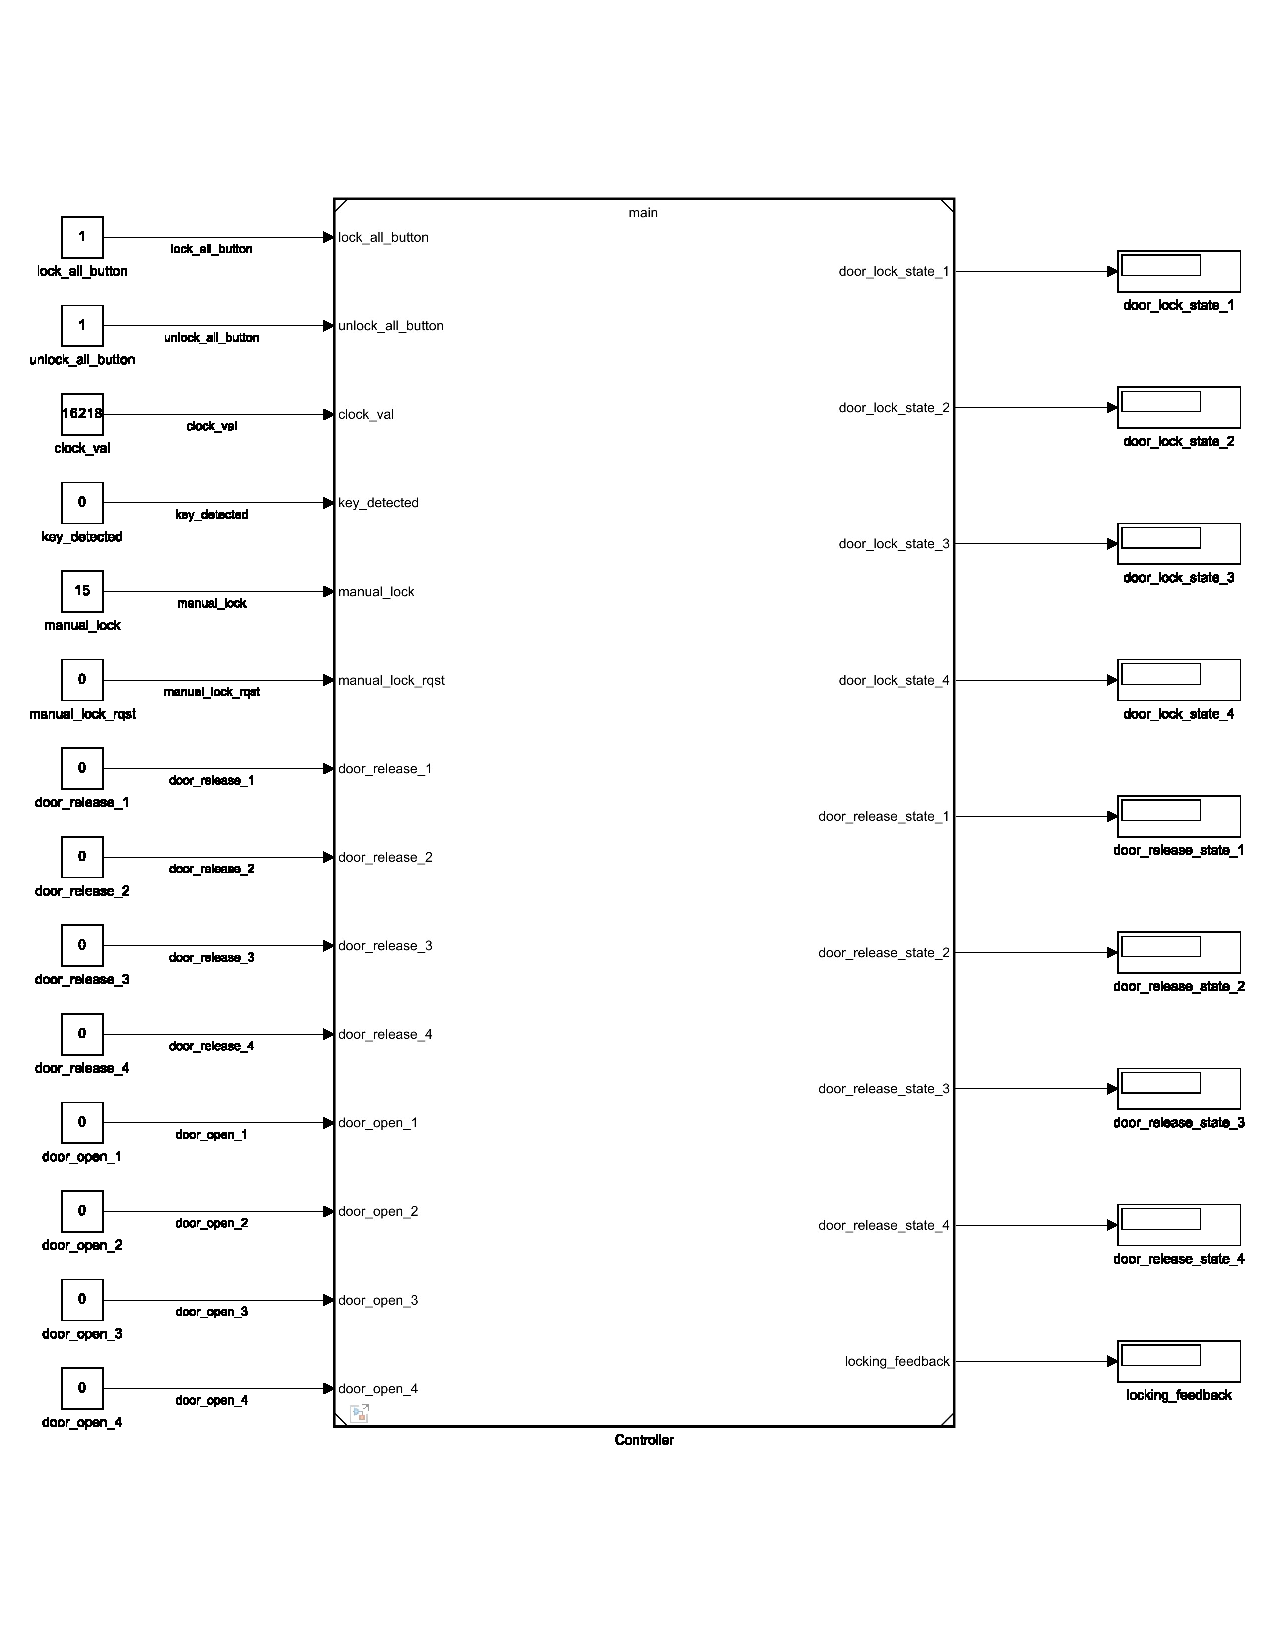
\includepdf[pages=-]{anexos/feature_model.pdf}

\end{anexosenv}


\end{document}
